\chapter{Developing the solution}

% Ada, Berners-Lee, Cerf, Dijkstra, Engelbart, Flowers, Gates, Hassabis, Ito, Jobs

\section{Sprint Ada}

This is Sprint Ada, the first iteration of my program. This iteration will be terminal-based, and mainly for creating the BFS implementation and adding in relevant functionality such as being able to enter multiple points, a basic visualisation etc.

\subsection{Tasks}

\begin{table}[htbp]
\centering
\begin{tabularx}{\textwidth}{|l|X|}
\hline
\textbf{Task ID} & \textbf{Task Description} \\
\hline
OCSP-001 & BFS Initialisation: Compare the representation methods available for BFS and then find a way to program that representation into the first version of the program. Main focus on a CLI and only 2 points \\
\hline
OCSP-002 & Terminal Visualisation: Create a basic visualisation of a path between 2 points in the terminal\\
\hline
OCSP-003 & Multi-point entry: Allow user to enter more than 2 points and find the shortest path between each, forming a large path from start to end. \\
\hline
\end{tabularx}
\end{table}

\subsection{Purpose}

This sprint entails me creating the first, basic algorithm for the SPA feature, and adding the multi-point entry so that it is useful in this scenario, as I intend for multiple items to be picked up at once.


\clearpage
\subsection{Sprint Planning Details}

\subsubsection{Technical Approach}

Breadth-First Search (BFS) was selected as the pathfinding algorithm for this stage. As the warehouse grid is currently unweighted (all moves have equal cost), BFS is guaranteed to find the shortest path in terms of the number of steps, directly meeting my stakeholders' core requirement for path optimisation. A* will be introduced at a later stage if time permits.

As this is still a very basic program focused solely on establishing the core BFS logic in the alpha stages of development, this prototype will start with procedural programming. This approach was chosen initially for speed of prototyping and simplicity, allowing focus entirely on the algorithm's correctness (addressing OCSP-001 core functionality) before introducing the structural overhead of OOP. Once the main BFS features have been confirmed to work and complexity increases with multi-point routing and visualisation, I will move to an object-oriented approach for better long-term structure, maintainability, and scalability.
\begin{enumerate}
    \item Create a 10 $\times$ 10 2D array to represent the graph.
    \item Define the start and end nodes.
    \item Initialize the queue with the start node.
    \item Create an empty set for visited nodes.
    \item Define possible movement directions (up, down, left, right).
    \item While the queue is not empty:
        \begin{enumerate}
            \item Pop the first path from the queue and \& get the last node in the current path.
            \item If the last node is the end node, return the current path.
            \item If the last node has not been visited, mark it as visited.
            \item For each possible direction:
                \begin{enumerate}
                    \item Calculate the new node.
                    \item If the new node is within bounds and not visited:
                        \begin{itemize}
                            \item Create a new path including the new node \& add the new path to the queue
                        \end{itemize}
                \end{enumerate}
        \end{enumerate}
    \item Create a function to repeat the pathfinding process for all points the user defines to find the shortest path between each pair of nodes. (OCSP-003)
    \item Display the path in a pretty format. (OCSP-002)
\end{enumerate}

\newpage


\subsubsection{Architecture \& Structural Considerations}

Below are the data structures I plan to use.
\begin{itemize}
    \item " Array (List of Lists): Representing the graph as a 10x10 2D array provides an easy abstraction of the warehouse layout. This structure was chosen for its simplicity and direct mapping to grid coordinates, making visualisation and boundary checks straightforward at this stage.
    \item Queue (using Python List): A standard Python list is used to implement the queue for BFS. While I could use \verb|collections.deque| due to O(1) appends/pops from both ends, I deemed the standard list sufficient for the current grid size and complexity. This will most likely change in future iterations as I make the solution more robust.
    \item Set (for Visited Nodes): A set is used to keep track of visited nodes. This provides an average of O(1) lookup time to check if a node has already been visited, preventing redundant exploration and cycles.
    \item List (for Paths/Directions): Lists store paths and directions; a list is the most suitable for appending nodes to paths during exploration as they are easy to use and easy to track via indexes.

\end{itemize}

\subsubsection{Dependencies}
There are no dependencies as such currently, I have opted to use Python's built-in functions (namely the list) for the queue rather than the external library \verb|queue| as mentioned above. This may change in future iterations if the code becomes too complex.

\newpage

\subsection{Development Summary}

\subsubsection{Iteration 1 - Hours: 3}
\begin{itemize}
    \item \textbf{Progress made:}
    \begin{itemize}
        \item OCSP-001: Created a fully working implementation of BFS that outputs the path it took, tested on a simple 10x10 grid.
        \item OCSP-002: Came up with an approach on how to output the path in a more interactive format, similar to the interface I presented in the usability section (see section X.X.X). I plan to use placeholder characters in the array to interpret the terminal output, as colours are not supported in most terminal emulators. [*] represents a user input point, and [=] represents the path taken.
    \end{itemize}
    \item \textbf{Blockers identified:}
    \begin{itemize}
        \item I used my knowledge from the CS50AI course to create the basic BFS implementation between 2 points. However, I struggled to think about how I could implement multiple points.

    \end{itemize}
    \item \textbf{Plan for next iteration:}
    \begin{itemize}
        \item Find a way to calculate the shortest path between more than 2 points.
        \item Add the visualisations using placeholder characters.
    \end{itemize}
\end{itemize}

\subsubsection{Iteration 2 - Hours: 1.5}
\begin{itemize}
    \item \textbf{Progress made:}
    \begin{itemize}
        \item OCSP-002: I completed the visualisation using my placeholder characters, displaying a grid in the terminal.
        \item OCSP-003: I managed to come up with an approach where the BFS algorithm is run between each pair of points, and the path is then connected together.
    \end{itemize}
    \item \textbf{Blockers identified:}
    \begin{itemize}
        \item I found that the grid did not display correctly as the user could not differentiate between their chosen points and the path followed. This was a very quick fix as I forgot to pass the 'points' parameter to the visualisation function to allow it to mark the points correctly.

    \end{itemize}
\end{itemize}

% Repeat daily log format for each development day

\clearpage
\subsection{Sprint Ada Implementation}

\subsubsection{Iteration 1: The BFS algorithm}

\textbf{Code Changes:}
\begin{itemize}
    \item \textbf{GitHub Commits:} d2fe05e, ad6ff95, e2c67a46
    \item \textbf{Explanation:}
    \begin{itemize}
        \item I enclosed the BFS algorithm in a function called \verb|bfs| with the parameters \verb|graph_in|, \verb|start| and \verb|end|. I originally intended to use consistent names, however Qodana flagged that this is not conventional. The naming scheme would have been in violation of PEP 3104, which addressed this issue. As such, I changed variable names like \verb|graph| to \verb|graph_in|, which is still an appropriate name (as it refers to the parameter being passed INto the function) but does not violate Python conventions.
        \item I chose a basic function structure for now, as I have only made a small part and single feature of my solution. However, I did implement sub-programs to organise my code better and allow for better debugging.
		\item As this was the first iteration, I annotated most lines of the code so I could easily pick up and trace the code. I made the comments relevant, descriptive but concise.
		\item This is a mostly standard BFS algorithm, with the modification of the data structure: I used a 2D array as it is an abstraction of a normal warehouse, applying the concept as defined in the Thinking Abstractly section.
    \end{itemize}
\end{itemize}

\textbf{Code Quality:}
\begin{itemize}
    \item \textbf{Annotations added:} As I was planning to continue this at a later time, I annotated each step of the BFS algorithm so that I could easily backtrack and visualise what was happening. I annotated most lines to ensure I would understand exactly how the algorithm worked and I could dry-run the algorithm in my head.
    \item \textbf{Variable/Structure naming:} I followed the lower-case underscore convention as defined by PEP 8. I focused on using industry terminology as my variable names, for example \verb|path| and \verb|node| 
    \item \textbf{Modular approach:} I have encapsulated all BFS-related code in a single BFS function. I have opted for this approach as BFS is a relatively simple algorithm, meaning the code is quite short and is appropriate to group into a single function.
\end{itemize}

\newpage

\subsubsection{Code Implementation:}
\begin{verbatim}
rows, cols = 10, 10
graph = [[0 for _ in range(cols)] for _ in range(rows)]

def bfs(graph_in, start, end):
    queue = [[start]] # Start with the start node
    visited = set() # Keep track of visited nodes
    directions = [(-1, 0), (1, 0), (0, -1), (0, 1)]  # Up, Down, Left, Right

    while queue:
        path = queue.pop(0) # Get the first path in the queue
        x, y = path[-1] # Get the last node in the path

        if (x, y) == end:
            return path # Return the path if we reach the end

        if (x, y) not in visited: # If the node has not been visited
            visited.add((x, y))  # Mark the node as visited
            for dx, dy in directions:  # Check all possible directions
                nx, ny = x + dx, y + dy  # Calculate the new node
                if 0 <= nx < rows and 0 <= ny < cols:  
                # Check if the new node is within the bounds
                    if (nx, ny) not in visited: 
                    # Check if the new node is not visited
                        new_path = list(path) + [(nx, ny)]  # Add new node to path
                        queue.append(new_path) # Add new path to queue

    return None  # Return None if no path is found


start_node = (0, 0)
end_node = (4, 8)

path = bfs(graph, start_node, end_node)
print(path)

\end{verbatim}

\newpage

\subsubsection{Dry Run}
This is a 'dry run' of the BFS algorithm I have made, to help visualise how the algorithm works.

\subsubsection{Initial Setup:}
\begin{itemize}
    \item Grid: $10 \times 10$ with all cells set to 0
    \item Start node: $(0,0)$
    \item End node: $(4,8)$
    \item Directions: Up $(-1,0)$, Down $(1,0)$, Left $(0,-1)$, Right $(0,1)$
\end{itemize}

\subsubsection{Step 1: Initialization}
\begin{itemize}
    \item Queue: $[[(0,0)]]$
    \item Visited: $\{\}$
\end{itemize}

\subsubsection{Step 2: First Iteration}
\begin{itemize}
    \item Pop first path from queue: $[(0,0)]$, Current position: $(0,0)$
    \item Check if current position is end: $(0,0) \neq (4,8)$, so continue
    \item Mark $(0,0)$ as visited: Visited = $\{(0,0)\}$
    \item Explore neighbours of $(0,0)$:
    \begin{itemize}
        \item Up: $(-1,0)$ - Out of bounds, skip
        \item Down: $(1,0)$ - Valid, not visited
        \begin{itemize}
            \item Add path $[(0,0), (1,0)]$ to queue
        \end{itemize}
        \item Left: $(0,-1)$ - Out of bounds, skip
        \item Right: $(0,1)$ - Valid, not visited
        \begin{itemize}
            \item Add path $[(0,0), (0,1)]$ to queue
        \end{itemize}
    \end{itemize}
    \item Queue: $[[(0,0), (1,0)], [(0,0), (0,1)]]$
\end{itemize}

\subsubsection{Step 3: Second Iteration}
\begin{itemize}
    \item Pop first path from queue: $[(0,0), (1,0)]$, Current position: $(1,0)$
    \item Check if current position is end: $(1,0) \neq (4,8)$, so continue
    \item Mark $(1,0)$ as visited: Visited = $\{(0,0), (1,0)\}$
    \item Explore neighbours of $(1,0)$:
    \begin{itemize}
        \item Up: $(0,0)$ - Already visited, skip
        \item Down: $(2,0)$ - Valid, not visited
        \begin{itemize}
            \item Add path $[(0,0), (1,0), (2,0)]$ to queue
        \end{itemize}
        \item Left: $(1,-1)$ - Out of bounds, skip
        \item Right: $(1,1)$ - Valid, not visited
        \begin{itemize}
            \item Add path $[(0,0), (1,0), (1,1)]$ to queue
        \end{itemize}
    \end{itemize}
    \item Queue: $[[(0,0), (0,1)], [(0,0), (1,0), (2,0)], [(0,0), (1,0), (1,1)]]$
\end{itemize}

\subsubsection{Step 4: Third Iteration}
\begin{itemize}
    \item Pop first path from queue: $[(0,0), (0,1)]$, Current position: $(0,1)$
    \item Check if current position is end: $(0,1) \neq (4,8)$, so continue
    \item Mark $(0,1)$ as visited: Visited = $\{(0,0), (1,0), (0,1)\}$
    \item Explore neighbours of $(0,1)$:
    \begin{itemize}
        \item Up: $(-1,1)$ - Out of bounds, skip
        \item Down: $(1,1)$ - Valid, not visited
        \begin{itemize}
            \item Add path $[(0,0), (0,1), (1,1)]$ to queue
        \end{itemize}
        \item Left: $(0,0)$ - Already visited, skip
        \item Right: $(0,2)$ - Valid, not visited
        \begin{itemize}
            \item Add path $[(0,0), (0,1), (0,2)]$ to queue
        \end{itemize}
    \end{itemize}
    \item Queue: $[[(0,0), (1,0), (2,0)], [(0,0), (1,0), (1,1)], [(0,0), (0,1), (1,1)], [(0,0), (0,1), (0,2)]]$
\end{itemize}

As the algorithm progresses, it explores all positions at distance 1 from start, then all positions at distance 2, then all positions at distance 3 and so on. The algorithm will eventually reach $(4,8)$ and return the path:
\begin{center}
$[(0,0), (1,0), (2,0), (3,0), (4,0), (4,1), (4,2), (4,3), (4,4), (4,5), (4,6), (4,7), (4,8)]$
\end{center}


\begin{figure}[htbp!]
    \centering
    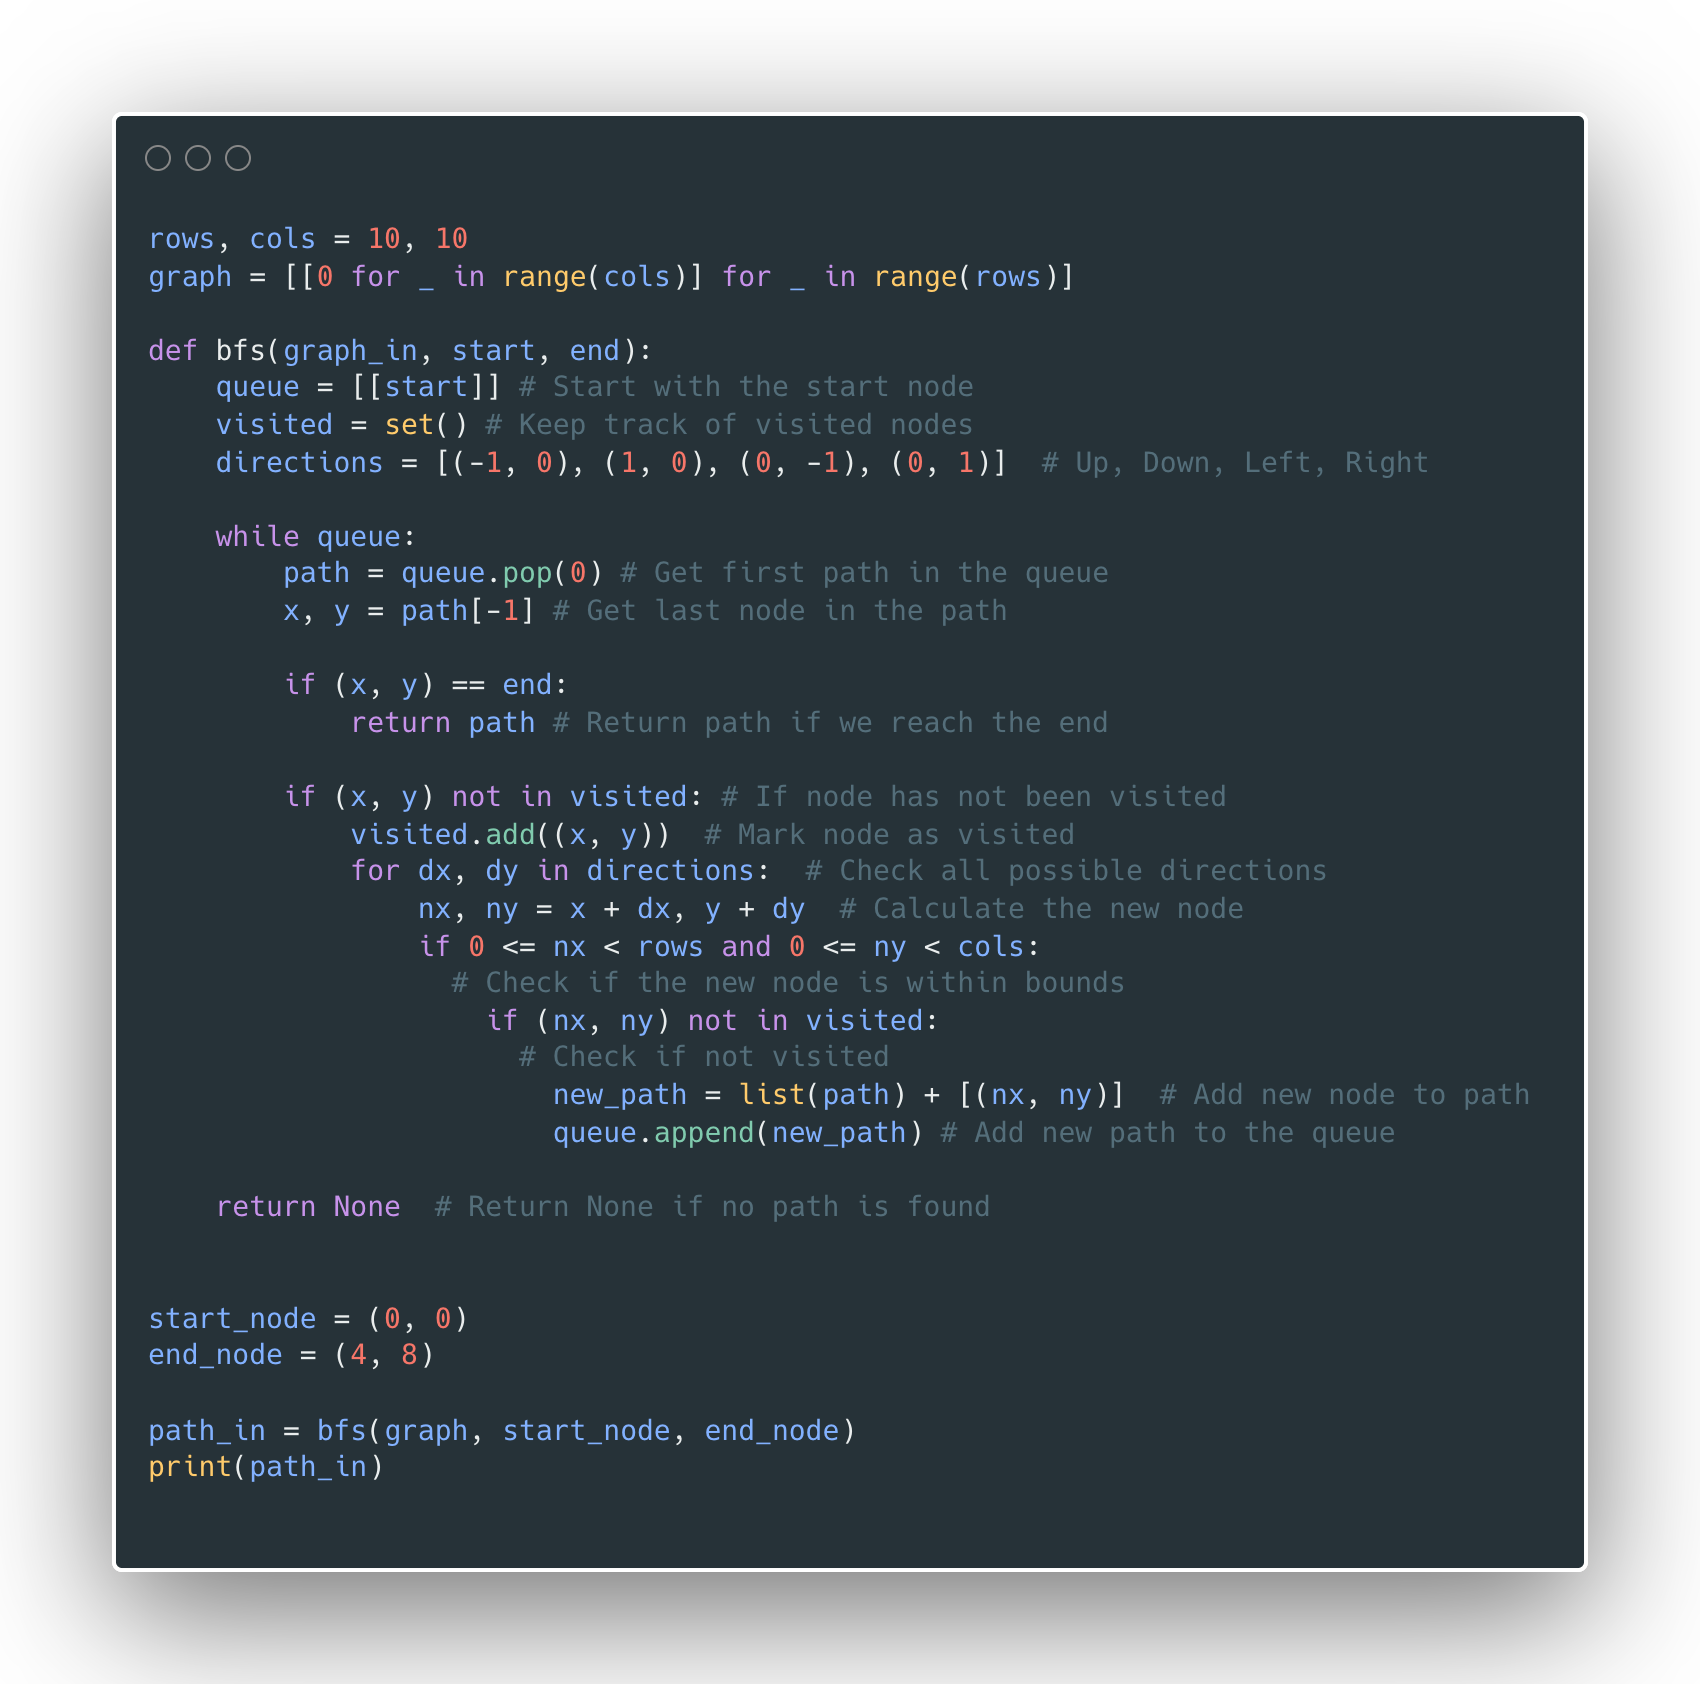
\includegraphics[width=1\linewidth]{Images/Source Code Image (2).png}
    \caption{A coloured screenshot of the code}
\end{figure}
\textbf{}\newline
\newpage

\subsubsection{Prototype details:} 
Currently, the BFS algorithm is working well for 2 defined points: a start and end node. It outputs a basic list of the coordinates that were followed to reach the end node from the start node. However, there is no visualisation as of yet, this will be implemented in the next iteration after some planning. As well as this, the BFS algorithm can currently handle only 2 points at a time, therefore I will be researching into how I can implement more points and allow the user to be able to set points to stop at.
\begin{figure}[htbp]
    \centering
    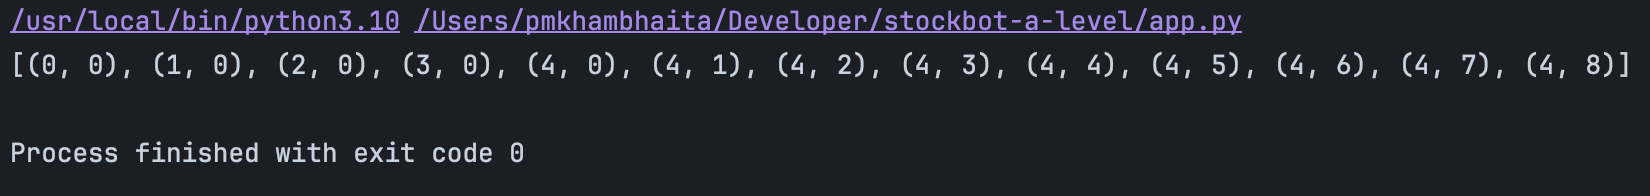
\includegraphics[width=0.8\textwidth]{Images/Screenshot 2025-03-30 at 11.18.52.png}
    \caption{The output of my algorithm with start at (0,0) and end at (4,8)}
\end{figure}

\subsubsection{Testing:}
\begin{table}[htbp]
\centering
\begin{tabularx}{\textwidth}{|l|X|p{3.5cm}|p{3.5cm}|c|}
\hline
\textbf{ID} & \textbf{Description} & \textbf{Expected} & \textbf{Actual} & \textbf{Pass?} \\
\hline
T1.1.1 & Input 0,0 and 9,9 & Direct path between both points & Direct path between points & X \\
\hline
T1.1.2 & Input 1,2 and 5,7 & Direct path between defined points only & Direct path between 1,2 and 5,7 & X \\
\hline
T1.1.3 & Input -1,-1 and 4,8 & Returns error & Error and break & \~{} \\
\hline
T1.1.4 & Input 0,1 and 10,10 & Return error & Error and break & \~{} \\
\hline

\end{tabularx}
\caption{Testing results for iteration 1}
\end{table}

\subsubsection{Tests justification}
These tests were for the main functionality of the program: the BFS must work because it is the heart of my program.
\subsubsection{Fixes}
T1.1.1 and T1.1.2 were successful, meaning the core functionality of the program is functional as expected. However, T1.1.3 and T1.1.4 were partially successful. While I did include the validation, I did not add a graceful error message, it was left to the basic python error-catching mechanisms. This will be fixed in the next iteration.

\newpage

\subsubsection{Screenshots of tests/program}

\begin{figure}[htbp!]
    \centering
    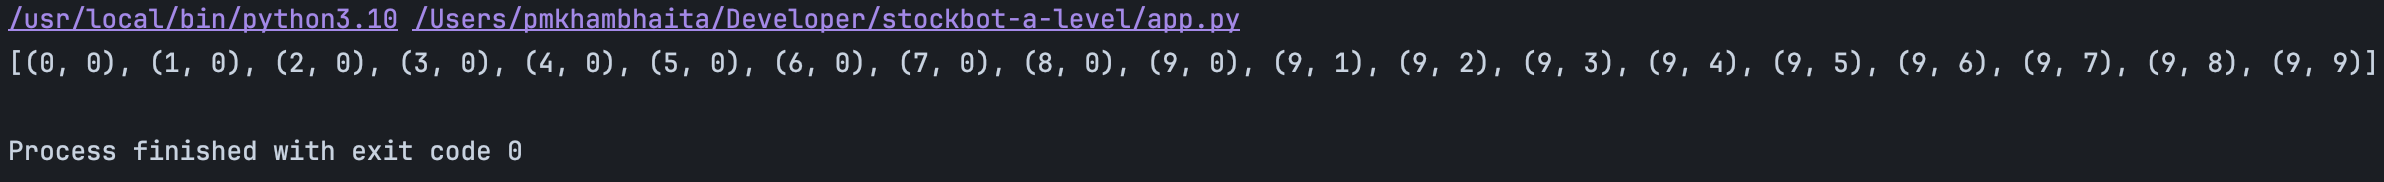
\includegraphics[width=1\linewidth]{Images/t1.1.png}
    \caption{T1.1.1 Output}
    \label{fig:enter-label}
\end{figure}

\begin{figure}[htbp!]
    \centering
    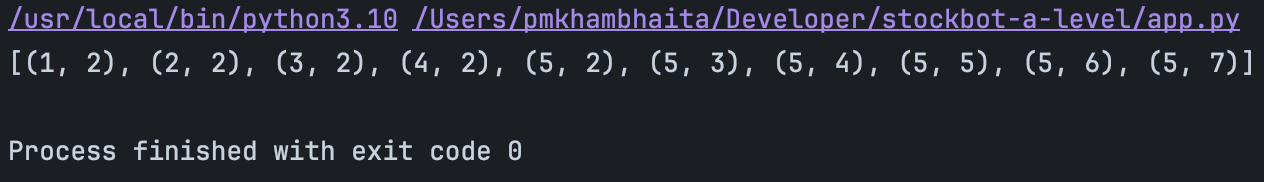
\includegraphics[width=1\linewidth]{Images/t1.2.png}
    \caption{T1.1.2 Output}
    \label{fig:enter-label}
\end{figure}

\begin{figure}[htbp!]
    \centering
    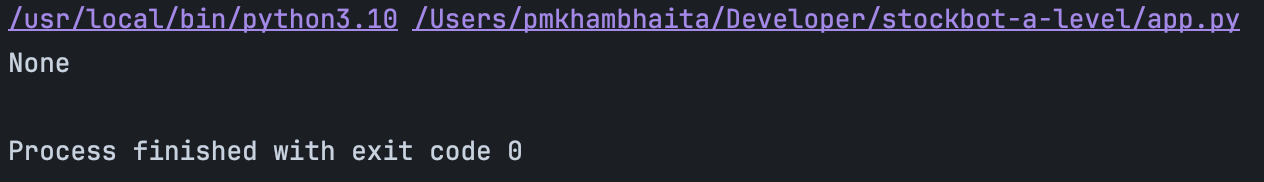
\includegraphics[width=1\linewidth]{Images/t1.3,1.4.png}
    \caption{T1.1.3 Output}
    \label{fig:enter-label}
\end{figure}

\begin{figure}[htbp!]
    \centering
    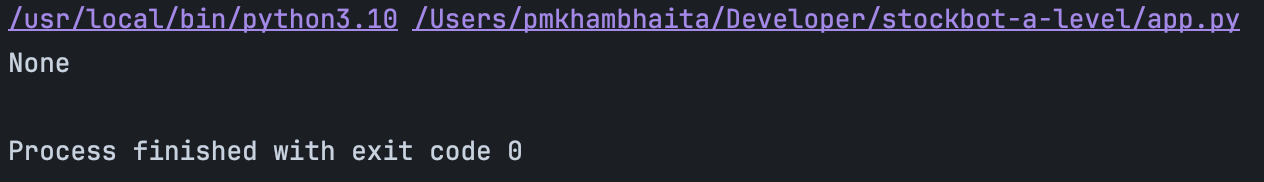
\includegraphics[width=1\linewidth]{Images/t1.3,1.4.png}
    \caption{T1.1.4 Output}
    \label{fig:enter-label}
\end{figure}

\newpage

\subsubsection{Validation:}
\begin{itemize}
    \item Boundary check: I ensured that the new node \verb|(nx, ny)| is within the bounds of the graph
    \item Visited check: I checked that the new node \verb|(nx, ny)| has not been visited before.
\end{itemize}

\subsubsection{Qodana Analysis}
    \begin{itemize}
        \item Issues identified: Shadowed name from outer scope
        \item Resolved issues: Modified variable name to prevent this
    \end{itemize}

\begin{figure}[htbp!]
    \centering
    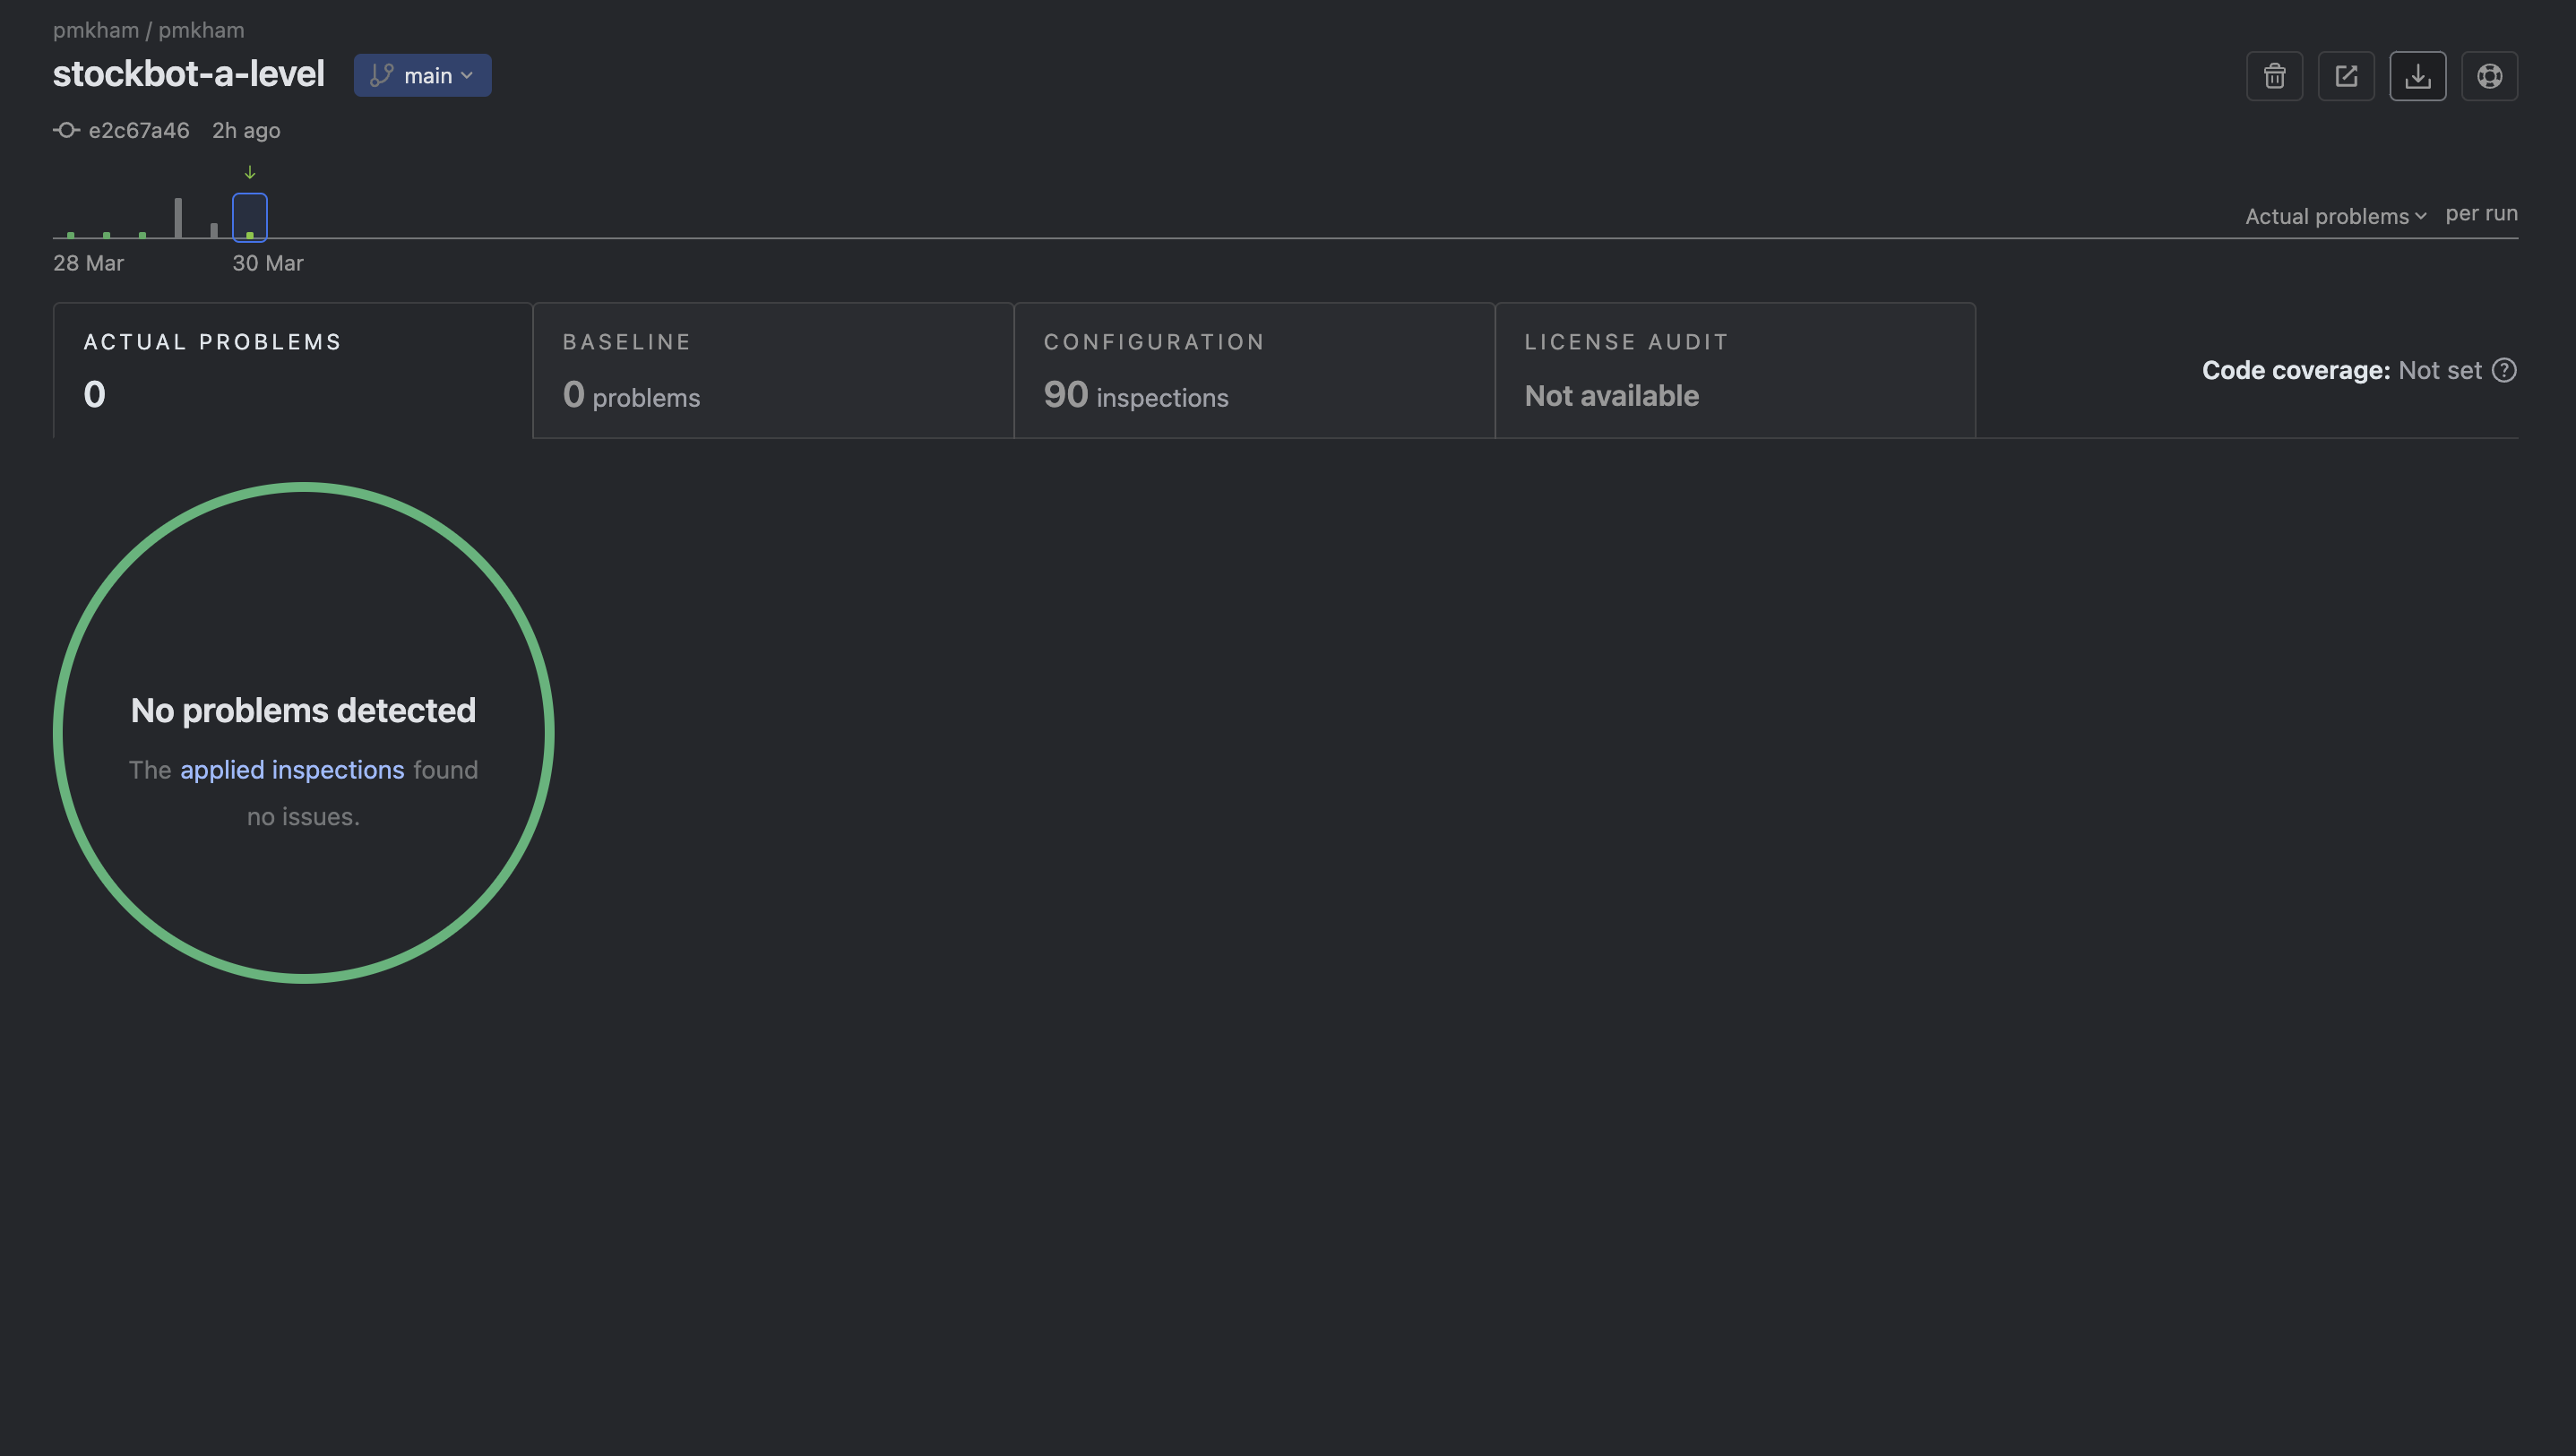
\includegraphics[width=1\linewidth]{Images/qodana-sai1.png}
    \caption{As of commit e2c67a46, no problems were identified.}
\end{figure}

\subsubsection{Review:}
\begin{itemize}
    \item Overall this iteration was quite successful. I managed to get a functional BFS algorithm working between 2 points, however I must be careful in not only validating but adding error messages for specific cases.
    \item Since this is still quite basic, I stuck to a simple procedural format rather than object-oriented principles. In the next iteration, I will be applying object-oriented principles as the program greatens in complexity.
\end{itemize}



\newpage

\subsubsection{Iteration 2: Multi-point BFS and Visualisation}

\textbf{Code Changes:}
\begin{itemize}
    \item \textbf{GitHub Commits:} c90ad6a, 7f76931, 9f2e44b, c88ec49, 94fef19, bc69274, 8081015, 0499de6
    \item \textbf{Explanation:}
    Reviewing Iteration 1 highlighted that managing the BFS logic, user input, potential future state (like obstacles), and visualisation within a single procedural script was becoming unwieldy. Specifically, integrating the multi-point logic (OCSP-003)  and the terminal visualisation (OCSP-002)  required passing numerous parameters between functions, increasing the risk of errors and making code harder to read and debug. Therefore, transitioning to an Object-Oriented approach in Iteration 2 was justified to encapsulate related data and behaviour (Grid state, Pathfinding logic, Visualisation) into distinct classes, improving modularity, testability, and preparing the structure for future feature additions like the GUI."
\end{itemize}

\textbf{Code Quality:}
\begin{itemize}
    \item \textbf{Annotations added:} I annotated key methods and classes with simple comments as to what they did and any program-specific syntax like my labelling scheme for the visualisation.

    \item \textbf{Modular approach:} I have now implemented an object-oriented approach in my solution, splitting the grid and pathfinder logic into 2 separate classes, referenced by outer functions that process user input and output.
\end{itemize}

\newpage

\subsubsection{Code Implementation:}

\lstinputlisting[style=custompython]{Code/sa2.py}


\begin{figure}[htbp!]
    \centering
    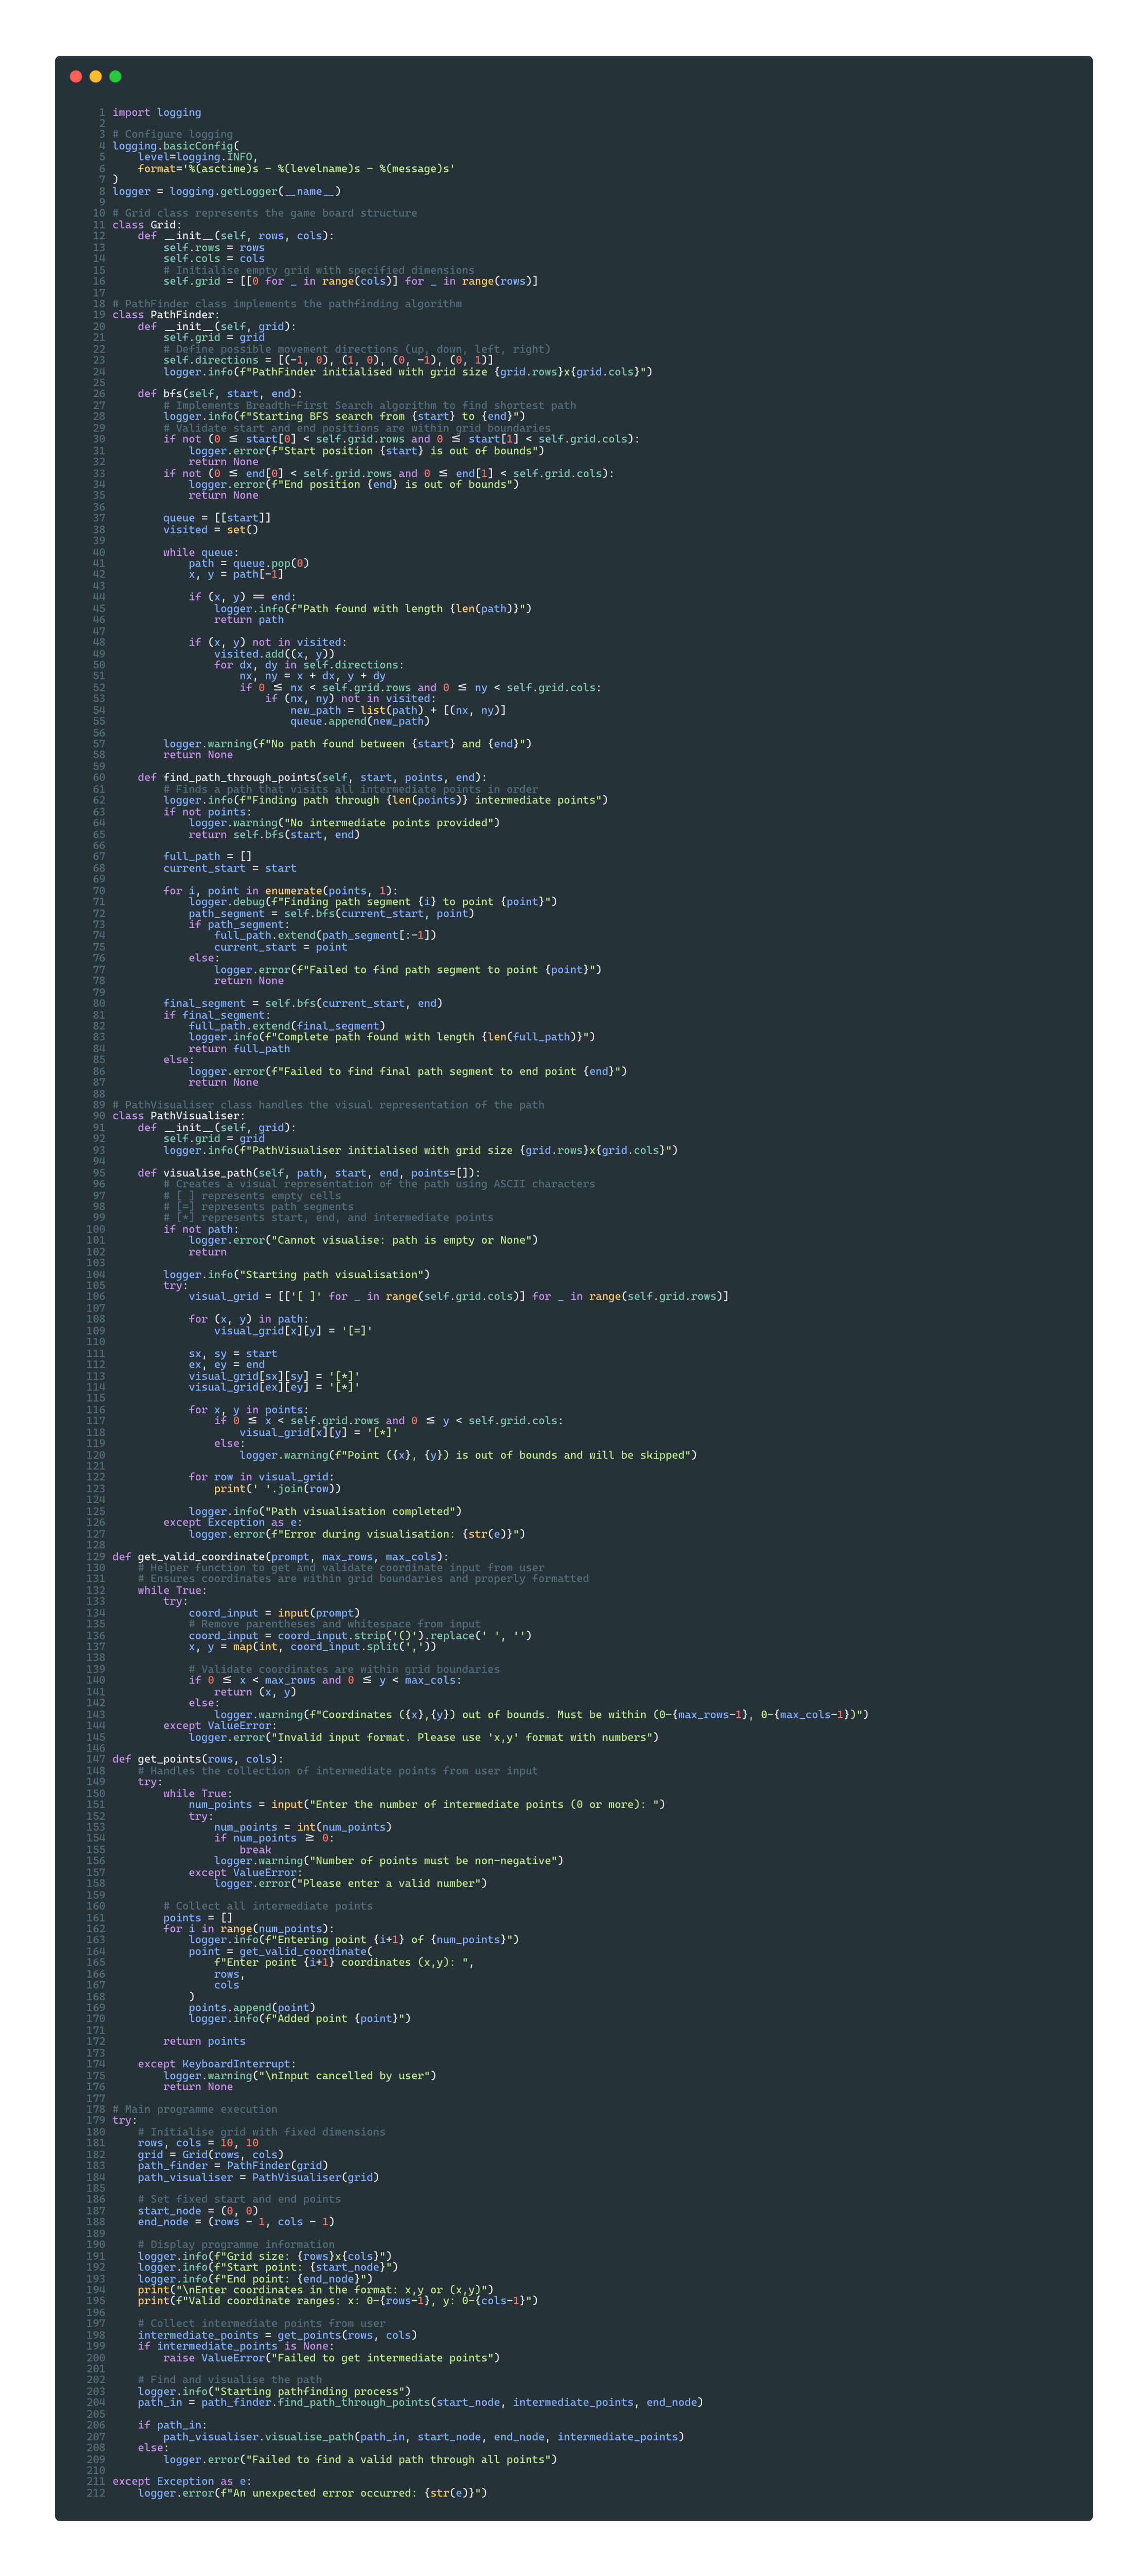
\includegraphics[width=0.61\linewidth]{Images/sa2.png}
    \caption{A coloured screenshot of the code}
\end{figure}
\textbf{}\newline
\newpage

\subsubsection{Prototype details:} 
The BFS algorithm is now working flawlessly, and I added some more debugging features like constant logging and output to the terminal using the \verb|logging| library within python. A timestamp and message is outputted when something of significance happens. The visualisation is also working excellently, and the user input is robust and easy to use. However, I do need to improve some parts of the logging, perhaps including the path the program will trace. As well as this, the path length is slightly inaccurate: it counts the start and end points, meaning it is 1 more than actual.

\begin{figure}[htbp]
    \centering
    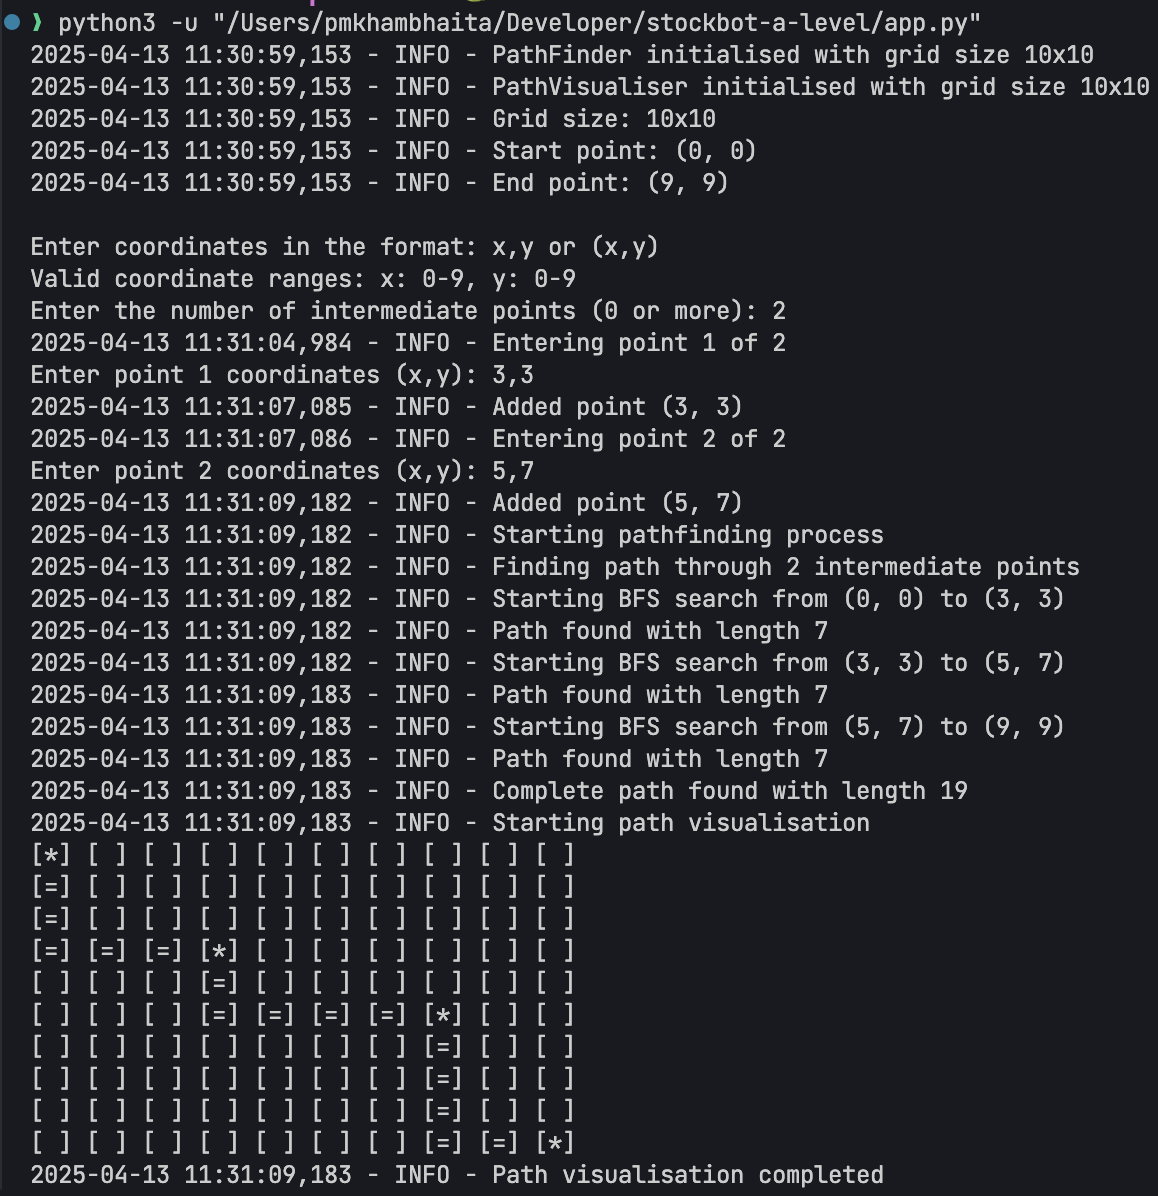
\includegraphics[width=0.8\textwidth]{Images/sa2test1.png}
    \caption{The output of my algorithm with points at (3,3) and end at (5,7)}
\end{figure}

\newpage

\subsubsection{Testing:}
\begin{table}[htbp]
\centering
\begin{tabularx}{\textwidth}{|l|X|p{3.5cm}|p{3.5cm}|c|}
\hline
\textbf{ID} & \textbf{Description} & \textbf{Expected} & \textbf{Actual} & \textbf{Pass?} \\
\hline
T1.2.1 & No intermediate points selected & Direct path between start and end & Direct path between start and end & X \\
\hline
T1.2.2 & Input 3,4 and 5,8 & Direct path between start and end stopping at defined points only & Direct path between start and end stopping at 3,4 and 5,8 & X \\
\hline
T1.2.3 & Input -1,-1 & Returns error & Returned graceful error and allowed retry & X \\
\hline
T1.2.4 & Input one valid and one non-valid point & Return error & Returned graceful error and allowed retry & X \\
\hline
T1.2.5 & Input 5 invalid points & Prevent entering from 1st points & Prevented addition of extra points until valid & X \\
\hline
T1.2.6 & Input valid points and verify it is the shortest path & Shortest path found & Shortest path found, path length incorrect & \~{} \\
\hline

\end{tabularx}
\caption{Testing results for iteration 1}
\end{table}

\subsubsection{Tests justification}
These tests were checking the validation measures I put in place for the SPA. These checked that all the validation was working, from boundary testing to existence validation. This was necessary to ensure the program is robust enough for the stakeholders and to cover all cases.


\subsubsection{Fixes}
Almost all tests were successful, and all previous errors have been resolved. However, the last test - T1.2.6 - was only a partial success - while the path was the shortest, the path length was out by +1. The issue was that the path length was being reported as the number of nodes in the path, but the actual path length should be the number of steps between nodes, which is one less than the number of nodes. Hence, I changed \verb|len(path)| to \verb|len(path) - 1|. This has been fixed in commit 121c011 and 1a7da80.

\newpage

\subsubsection{Screenshots of tests/program}

\begin{figure}[htbp!]
    \centering
    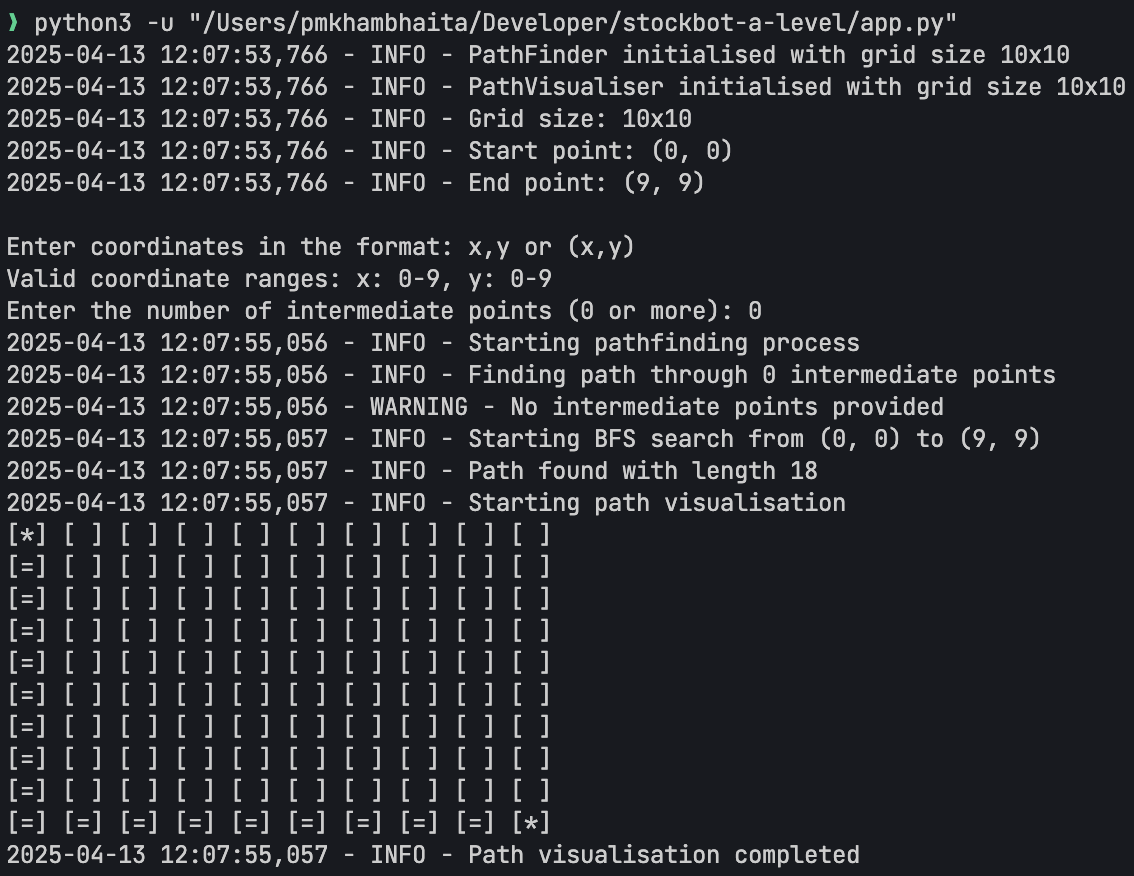
\includegraphics[width=1\linewidth]{Images/t1.2.1.png}
    \caption{T1.2.1 Output}
    \label{fig:enter-label}
\end{figure}

\begin{figure}[htbp!]
    \centering
    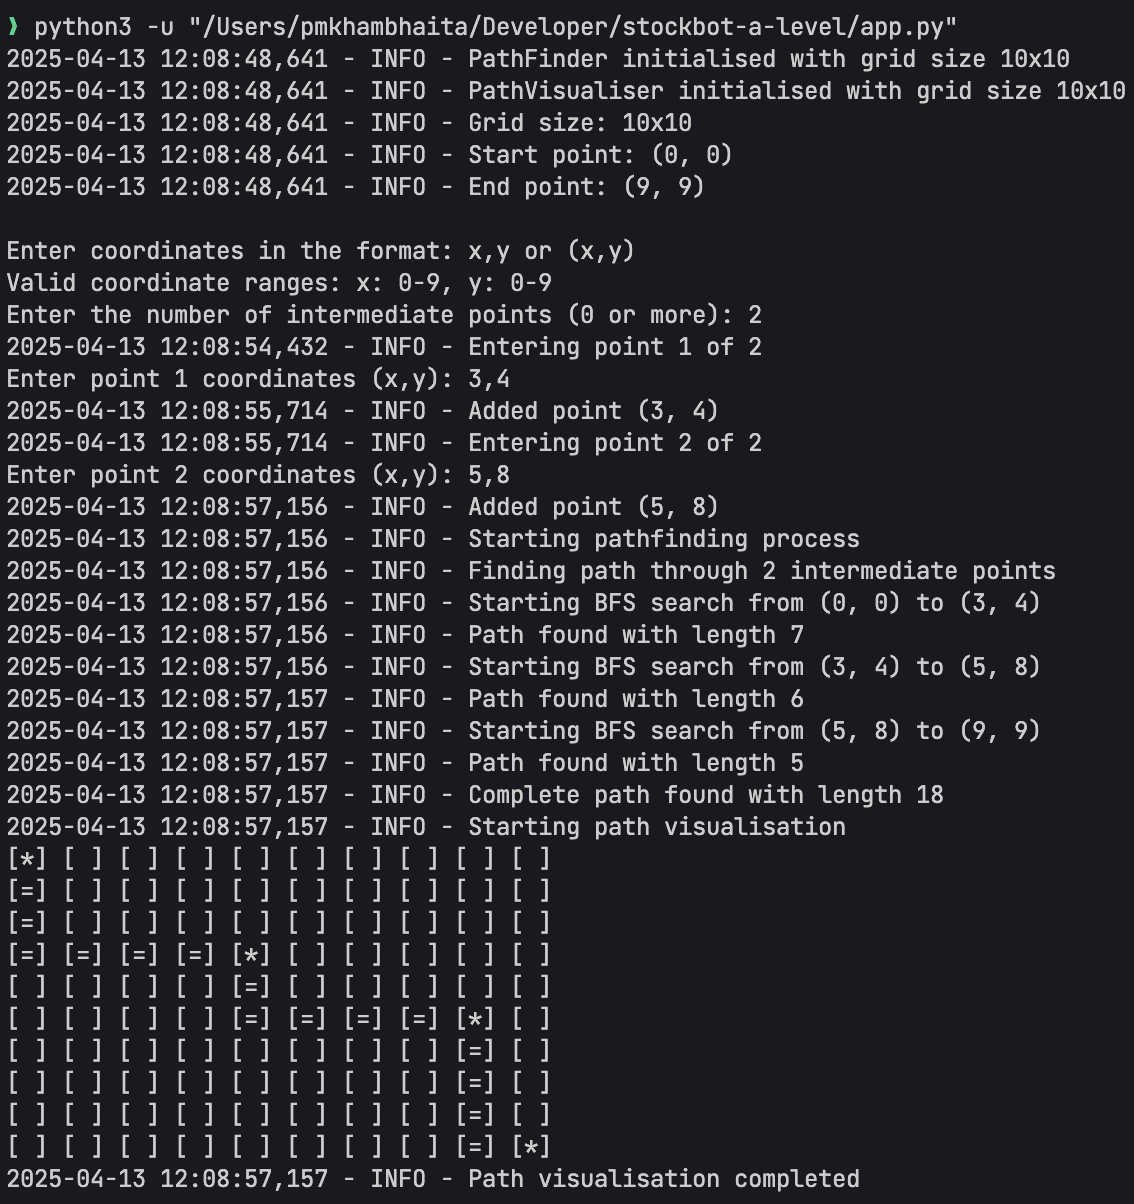
\includegraphics[width=1\linewidth]{Images/t1.2.2.png}
    \caption{T1.2.2 Output}
    \label{fig:enter-label}
\end{figure}

\begin{figure}[htbp!]
    \centering
    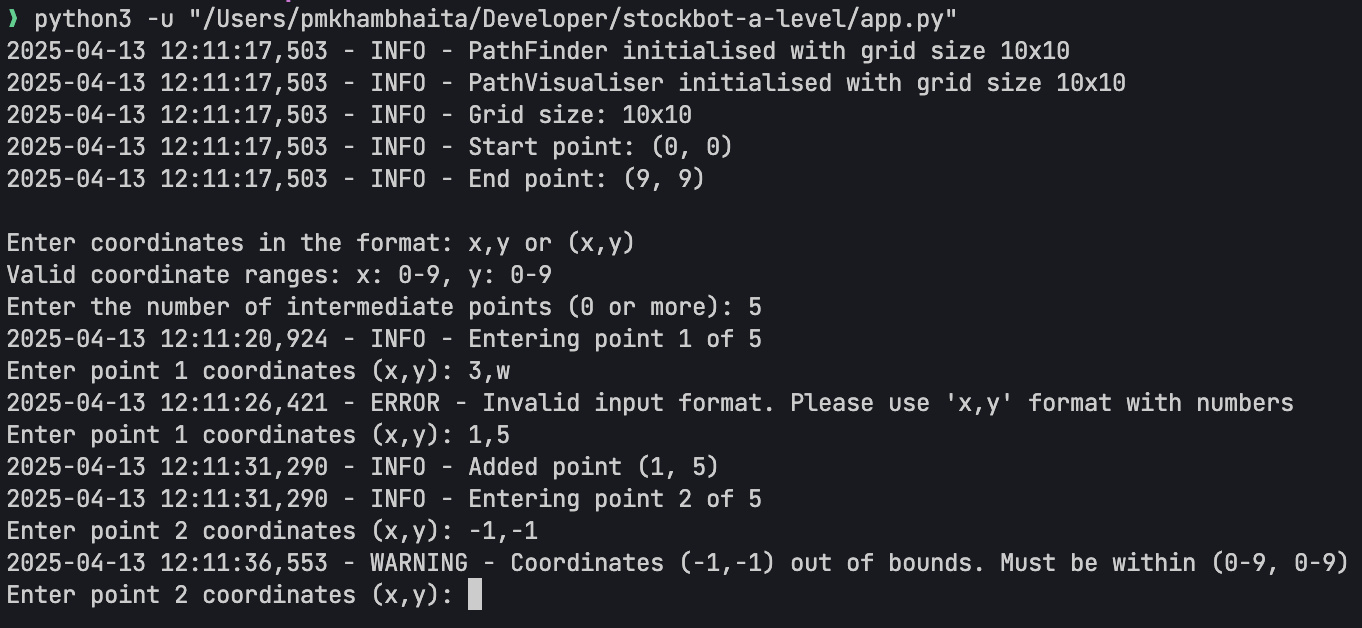
\includegraphics[width=1\linewidth]{Images/t1.2.x.png}
    \caption{T1.2.3/4/5 Output}
    \label{fig:enter-label}
\end{figure}

\begin{figure}[htbp!]
    \centering
    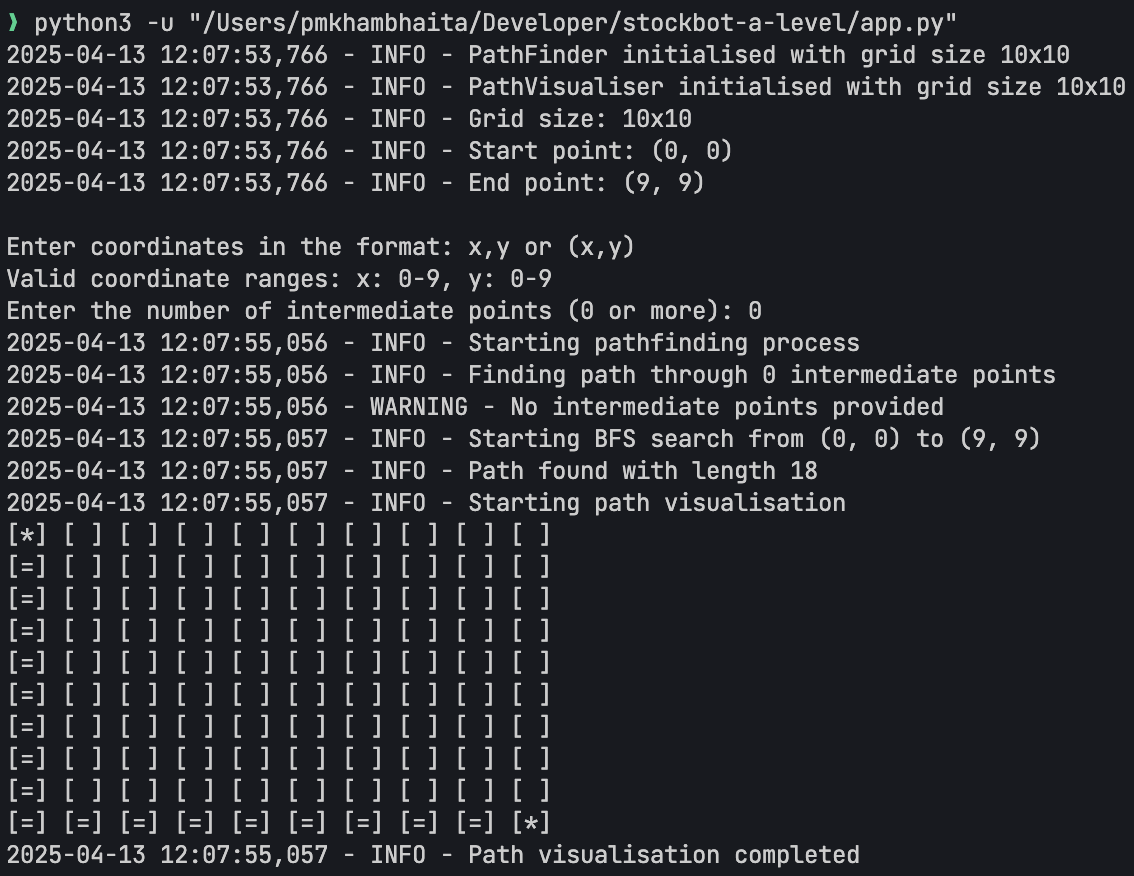
\includegraphics[width=1\linewidth]{Images/t1.2.1.png}
    \caption{T1.2.6 Output (fixed)}
    \label{fig:enter-label}
\end{figure}

\newpage

\subsubsection{Validation:}
\begin{itemize}
    \item \textbf{User input boundary \& range validation} - Confirms all user-provided points are within the grid boundaries and valid range of 0-9.
    \item \textbf{Type \& format validation} - Ensures coordinates are entered in the correct format (x,y) and contain valid numbers
    \item \textbf{Number of points validation} - Checks that the number of intermediate points entered is a non-negative integer
    \item \textbf{Path visualisation validation} - Confirms a path exists before attempting to visualise it
    \item \textbf{User point existence validation} - Handles the case where no intermediate points are provided
    \item \textbf{Exception handling} - Catches and logs any unexpected errors during program execution
\end{itemize}

\subsubsection{Qodana Analysis}
   I resolved all of the issues flagged by Qodana in commit c78f7fc6. Most of the errors were shadwing names from outer scopes, so I used the refactor function in my IDE to fix these issues.

\begin{figure}[htbp!]
    \centering
    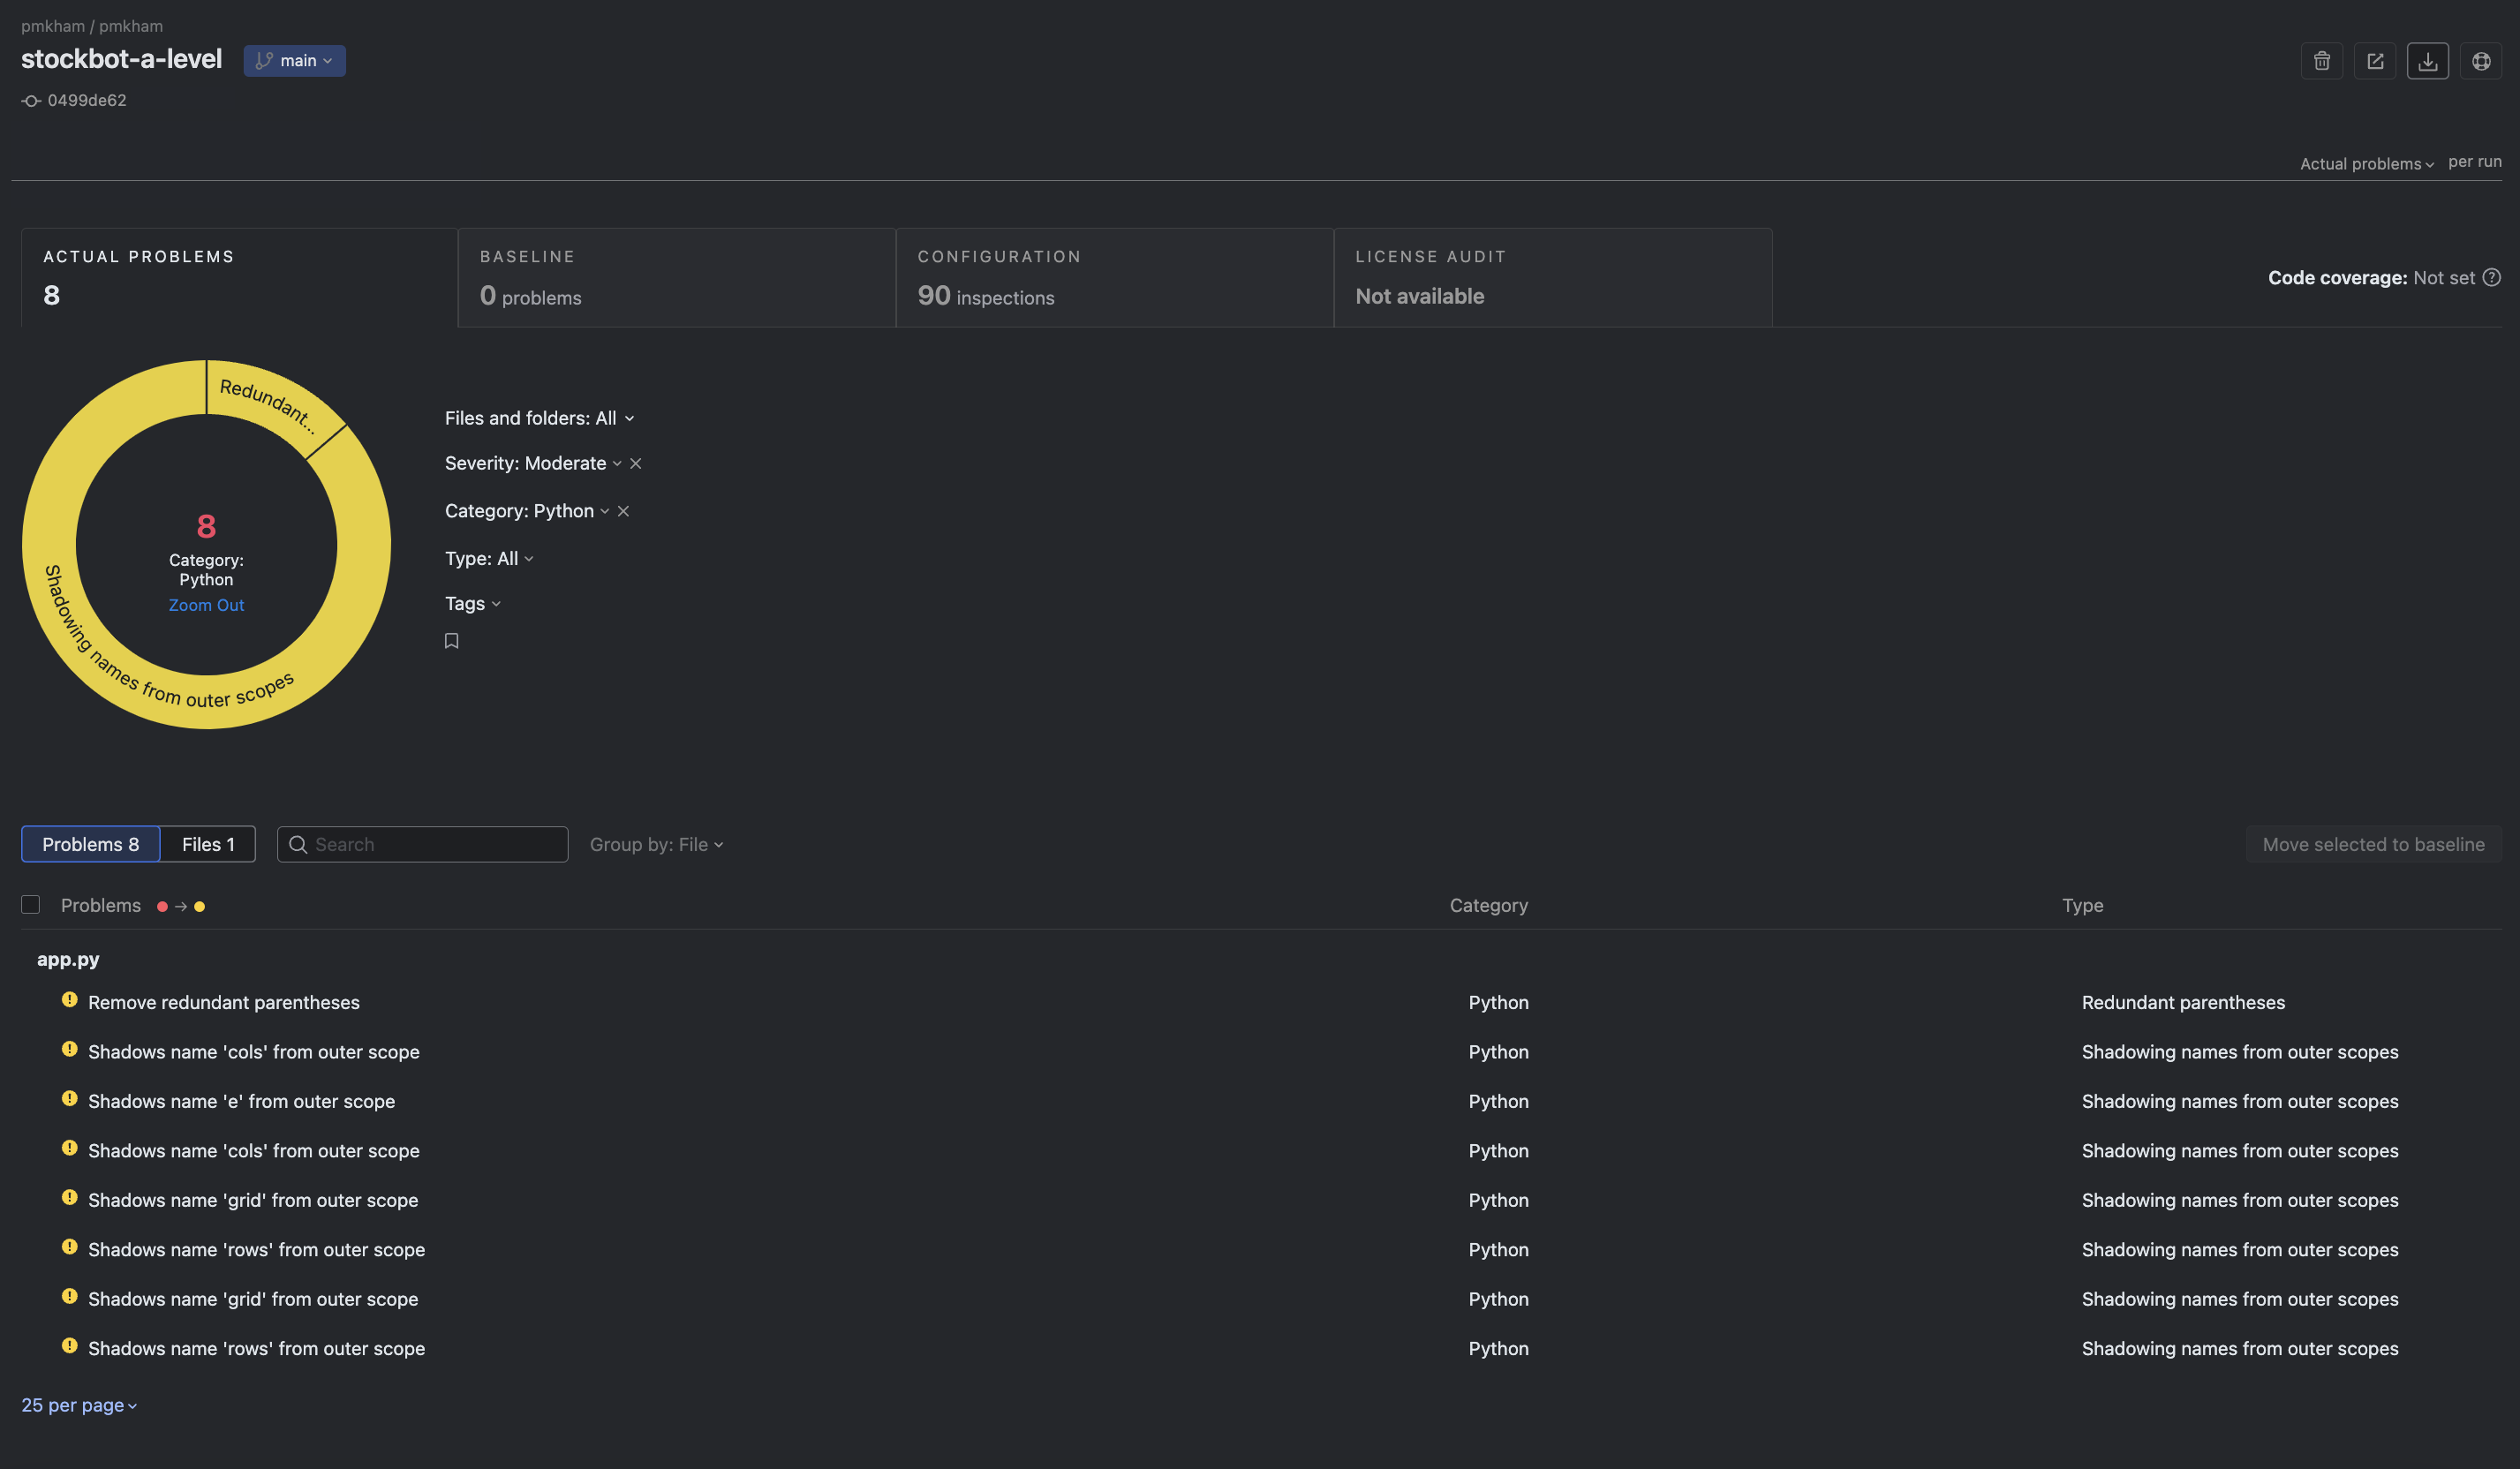
\includegraphics[width=0.85\linewidth]{Images/qodana-sa2.png}
    \caption{As of commit 1a7da80, 8 problems were identified.}
\end{figure}

\subsubsection{Review:}
 Overall this iteration was very successful. I have now completed what I set out to do in this sprint. There were some minor errors along the way, but they were fixed very quickly: they were mainly logic errors rather than syntax.

\clearpage
\subsection{Sprint Review and Retrospective}

\subsubsection{Accomplishments}
\begin{itemize}
    \item Completed OCSP-001 to OCSP-003
    \item  I have now successfully implemented the shortest path feature of my program, and is ready to use. Hence, the first stage of my design - getting a functional SPA running - is complete.
\end{itemize}

\subsubsection{Final testing}

This testing is performed by my stakeholders; they each came up with 1 test they would like to perform in person. This testing  conducted using the data provided in Section x.x.x. In this case, since this program has only implemented the SPA, they will only be using the respective criteria:

\begin{itemize}
\item Grid is 15 x 15
\item Points using random num gen between 0 and 14 (x2): (2,5), (8,9), (10,2) 

\end{itemize}

\begin{table}[htbp]
\centering
\begin{tabularx}{\textwidth}{|l|X|p{3.5cm}|p{3.5cm}|c|}
\hline
\textbf{ID} & \textbf{Description} & \textbf{Expected} & \textbf{Actual} & \textbf{Pass?} \\
\hline
T1.F.1 & Path found using input points & Path between start and end including user-defined points& Direct path between start and end stopping at (2,5), (8,9) and (10,2)  & X \\
\hline
T1.F.2 & Input invalid points (letters, numbers and symbols) & Warns user that points are invalid & Prevents user from entering the points and displays a descriptive message & X \\
\hline
T1.F.3 & Input no points &  Direct path between start and end & Direct path between start and end & X \\
\hline
\end{tabularx}
\end{table}

\subsubsection{Testing Summary}
\begin{table}[htbp]
\centering
\begin{tabular}{|l|c|}
\hline
\textbf{Metric} & \textbf{Count} \\
\hline
Total tests conducted & 13 \\
\hline
Tests passed & 11 \\
\hline
Tests failed & 2 \\
\hline
Fixed issues & 3 \\
\hline
\end{tabular}
\caption{Sprint 1 testing summary}
\end{table}

\newpage

\subsubsection{Validation}
    \begin{itemize}
    \item \textbf{Grid Boundary Validation for Start/End Points} - Checks if coordinates are within grid dimensions
    \item \textbf{User Input Format Validation} - Validates coordinate input format (x,y)
    \item \textbf{User Input Range Validation} - Confirms coordinates are within valid grid dimensions
    \item \textbf{Number of Points Validation} - Ensures number of intermediate points is non-negative
    \item \textbf{Path Existence Validation} - Verifies if a valid path exists between points
    \item \textbf{Intermediate Point Boundary Validation} - Ensures user-provided points are within grid boundaries
    \item \textbf{Path Visualisation Validation} - Checks if a path exists before attempting visualisation
\end{itemize}

\subsubsection{Robustness}
\begin{itemize}
    \item \textbf{Exception Handling} -- Uses try-except blocks to catch and log unexpected errors
    \item \textbf{Logging Implementation} -- Comprehensive logging of program flow and errors
    \item \textbf{Default Parameter Values} -- Uses None as default for optional parameters
    \item \textbf{Queue Management in BFS} -- Properly manages the queue in breadth-first search
    \item \textbf{Path Segment Validation} -- Validates each segment of the multi-point path
    \item \textbf{Keyboard Interrupt Handling} -- Catches user interruptions during input collection
    \item \textbf{Consistent Return Values} -- Functions return None for failure cases
    \item \textbf{Empty Points List Handling} -- Gracefully handles cases with no intermediate points
\end{itemize}


\subsubsection{Link}

With the completion of this sprint, I have now created one complete feature that was requested by the stakeholders: the shortest path algorithm. From the design section, I have successfully implemented BFS to shorten the time taken to collect items, which means I have met one of the requirements from the stakeholders. This is because BFS has significantly reduced the time taken to find an optimal path, the main purpose of my solution. \newline The next sprint will focus on creating the GUI and adding more usability features to make the program easy to use: currently it is still terminal-based. (see the design breakdown)


\clearpage

% Berners-Lee

\section{Sprint Berners-Lee}

This is Sprint Berners-Lee, the second iteration of my program. This iteration focuses on developing the Graphical User Interface (GUI) using Tkinter, replacing the previous terminal-based interaction. The goal is to provide a user-friendly way to input points and visualise the shortest path generated by the existing SPA (Shortest Path Algorithm) logic.

\subsection{Tasks}

\begin{table}[htbp]
	\centering
	\begin{tabularx}{\textwidth}{|l|X|}
		\hline
		\textbf{Task ID} & \textbf{Task Description} \\
		\hline
		OCSP-004 & Project Restructure: Reorganise code by separating GUI logic (\verb|gui.py|) from the core pathfinding logic (\verb|spa.py|) for better modularity. \\
		\hline
		OCSP-005 & GUI Scaffolding: Create the basic Tkinter window structure, input fields (point entry), output area (text box), and control buttons (\verb|Add Point|, \verb|Find Path|, \verb|Clear|). Implement layout using the \verb|grid| manager. \\
		\hline
		OCSP-006 & GUI-SPA Integration: Connect GUI elements to the backend \verb|spa.py| classes (\verb|Grid|, \verb|PathFinder|, \verb|PathVisualiser|). Implement functionality for adding points, triggering pathfinding, and clearing inputs via button clicks. \\
		\hline
		OCSP-007 & Visualisation Output Redirection: Capture the standard output of the \verb|visualise_path| method (which previously printed to terminal) and display it within the GUI's text output area. \\
		\hline
		OCSP-008 & Validation Integration \& Error Handling: Implement robust input validation within the GUI, preventing invalid coordinates (out of bounds, start/end points, incorrect format) and providing clear error messages directly in the GUI output area. Remove redundant terminal-based input functions. \\
		\hline
		OCSP-009 & Logging Enhancement: Implement logging to a dedicated file (\verb|stockbot_log.txt|) alongside terminal logging for persistent debugging information. \\
		\hline
		OCSP-010 & GUI Refinements: Improve clarity of error messages, ensure GUI starts cleanly without residual terminal interactions, and add a textual representation of the path sequence to the output. \\
		\hline
	\end{tabularx}
\end{table}

\subsection{Purpose}

This sprint aims to significantly enhance usability by transitioning from a command-line interface to a graphical one. This addresses the need for a more intuitive user experience, allowing users to easily input intermediate points and view the calculated shortest path, including a visual grid representation, directly within a dedicated application window. This aligns with the project goal of creating an accessible tool for warehouse path optimisation.

\clearpage
\subsection{Sprint Planning Details}

\subsubsection{Technical Approach}

The primary technology chosen for the GUI is Python's built-in \verb|Tkinter| library, ensuring minimal external dependencies. The development followed these steps:

\begin{enumerate}
	\item \textbf{Restructure:} Separate existing SPA logic (\verb|app.py| renamed to \verb|spa.py|) from new GUI code (\verb|gui.py|). This promotes modularity and adheres to the Single Responsibility Principle. (OCSP-004)
	\item \textbf{GUI Layout:} Utilise Tkinter's \verb|grid| geometry manager for flexible and organised placement of widgets (Frames, Entry, Button, Text). (OCSP-005)
	\item \textbf{Component Initialisation:} Instantiate necessary classes from \verb|spa.py| within the \verb|PathfinderGUI| class (\verb|Grid|, \verb|PathFinder|, \verb|PathVisualiser|). (OCSP-006)
	\item \textbf{Event Handling:} Implement methods (\verb|add_point|, \verb|find_path|, \verb|clear_all|) triggered by button clicks. (OCSP-006)
	\item \textbf{Input Handling:} Retrieve and parse user input from the \verb|ttk.Entry| widget. (OCSP-006)
	\item \textbf{Output Redirection:} Use \verb|io.StringIO| and \verb|sys.stdout| redirection to capture the printed output of \verb|path_visualiser.visualise_path| and insert it into the \verb|tk.Text| widget. (OCSP-007)
	\item \textbf{Validation:} Implement a dedicated validation function (\verb|validate_point| in \verb|spa.py|) checking boundaries and start/end point exclusion. Call this function from the GUI's \verb|add_point| method. Display validation errors directly in the GUI's output text area. Remove old terminal input functions (\verb|get_valid_coordinate|, \verb|get_points|) from \verb|spa.py|. (OCSP-008)
	\item \textbf{Logging:} Configure the \verb|logging| module in \verb|spa.py| to add a \verb|FileHandler|, directing logs to \verb|stockbot_log.txt| in addition to the console. (OCSP-009)
	\item \textbf{Refinements:} Improve error message wording for clarity. Add textual path sequence output (\verb|(0,0) -> (1,0) -> ...|) to the GUI. Ensure the main execution block in \verb|spa.py| (which previously ran the terminal version) is removed to prevent interference. (OCSP-010)
\end{enumerate}

\subsubsection{Architecture \& Structural Considerations}

The architecture now consists of two main Python files:
\begin{itemize}
	\item \verb|spa.py|: Contains the backend logic classes (\verb|Grid|, \verb|PathFinder|, \verb|PathVisualiser|) and helper functions (\verb|validate_point|). It also handles logging configuration. The classes remain largely unchanged from Sprint Ada, ensuring the core pathfinding algorithm is stable.
	\item \verb|gui.py|: Introduces the \verb|PathfinderGUI| class, responsible for creating and managing all Tkinter widgets. It orchestrates user interaction, calling methods from \verb|spa.py| for validation and pathfinding, and displaying results. It maintains the list of user-added points (\verb|self.points|).
\end{itemize}
This separation allows for independent development and testing of the backend logic and the user interface.

\subsubsection{Dependencies}
This sprint introduces a dependency on Python's standard \verb|Tkinter| library for the GUI. Standard libraries \verb|io| and \verb|sys| are used for output redirection. The \verb|logging| library continues to be used.

\newpage

\subsection{Development Summary}
*(Note: Hours are estimated based on commit timestamps. Please adjust if you have accurate logs.)*

\subsubsection{Iteration 1 (Approx. 15 mins: ~14:35 - ~14:50)}
\begin{itemize}
	\item \textbf{Progress made:}
	\begin{itemize}
		\item OCSP-004: Restructured project, separating \verb|gui.py| and \verb|spa.py|.
		\item OCSP-005: Set up basic Tkinter window (\verb|PathfinderGUI| class), configured \verb|grid| layout manager, added input entry, output text area, and control buttons.
		\item OCSP-006 (Partial): Initialised backend components (\verb|Grid|, \verb|PathFinder|, etc.) within the GUI class method \verb|__init__|. Implemented basic \verb|add_point|, \verb|find_path|, \verb|clear_all| methods and linked them to buttons. Connected \verb|add_point| to basic boundary check and \verb|find_path| to call the backend pathfinding.
		\item OCSP-007: Implemented output redirection using \verb|io.StringIO| to display the visualiser's grid output in the GUI text area.
	\end{itemize}
	\item \textbf{Blockers identified:}
	\begin{itemize}
		\item The terminal interface defined in \verb|spa.py|'s main execution block was still running alongside the GUI.
		\item Basic validation allowed adding start/end points (0,0 or 9,9) as intermediate points.
		\item Error messages were logged to the terminal via \verb|spa.logger| but not displayed within the GUI itself.
	\end{itemize}
	\item \textbf{Plan for next iteration:}
	\begin{itemize}
		\item Remove residual terminal code execution from \verb|spa.py|.
		\item Implement stricter validation to prevent adding start/end points.
		\item Integrate error/warning messages directly into the GUI output area.
	\end{itemize}
\end{itemize}

\subsubsection{Iteration 2 (Approx. 5 mins: ~14:50 - ~14:55)}
\begin{itemize}
	\item \textbf{Progress made:}
	\begin{itemize}
		\item OCSP-008 (Partial): Created \verb|validate_point| function in \verb|spa.py| to check boundaries AND prevent adding start/end points. Modified GUI \verb|add_point| to use this new function. Removed old terminal input functions (\verb|get_valid_coordinate|, \verb|get_points|) and main execution block from \verb|spa.py|, resolving the simultaneous terminal/GUI execution issue.
		\item OCSP-009: Configured logging in \verb|spa.py| to output to \verb|stockbot_log.txt|.
		\item OCSP-008 (Partial) / OCSP-010 (Partial): Modified GUI methods (\verb|add_point|, \verb|find_path|) to display error messages (invalid format, no points added, validation failures) directly in the \verb|output_text| widget instead of just logging.
	\end{itemize}
	\item \textbf{Blockers identified:}
	\begin{itemize}
		\item Error message wording could be more user-friendly/specific (e.g., format error message).
		\item The GUI shows the visual grid path but doesn't list the sequence of coordinates followed.
	\end{itemize}
	\item \textbf{Plan for next iteration:}
	\begin{itemize}
		\item Refine error message text for better clarity.
		\item Add the sequence of path coordinates to the output.
	\end{itemize}
\end{itemize}

\subsubsection{Iteration 3 (Approx. 2 mins: ~14:55 - ~14:57)}
\begin{itemize}
	\item \textbf{Progress made:}
	\begin{itemize}
		\item OCSP-010: Improved error messages in \verb|gui.py| for invalid format, start/end point conflict, and out-of-bounds errors to be more intuitive. Made the "no points added" error more specific.
		\item OCSP-010: Added functionality to display the textual sequence of the path coordinates (e.g., \verb|(0,0) -> (1,0) -> ...|) in the GUI output area after the grid visualisation.
	\end{itemize}
	\item \textbf{Blockers identified:}
	\begin{itemize}
		\item None identified in this iteration; core GUI functionality complete for this sprint.
	\end{itemize}
\end{itemize}

\clearpage
\subsection{Sprint Berners-Lee Implementation}

\subsubsection{Iteration 1: Getting GUI Working}

\textbf{Code Changes:}
\begin{itemize}
	\item \textbf{GitHub Commits:} \verb|dc29116|, \verb|51caad0|, \verb|2cc86ce|, \verb|93cddaa|, \verb|256e1a2| (partially - validation function creation), \verb|be7179a| (partially - removing terminal execution)
	\item \textbf{Explanation:}
	\begin{itemize}
		\item Project structure was refactored by creating \verb|gui.py| for Tkinter code and renaming \verb|app.py| to \verb|spa.py| to hold the backend logic. This separation improves organisation.
		\item The basic \verb|PathfinderGUI| class was created using Tkinter. The window layout was defined using the \verb|grid| manager for better control over widget placement compared to \verb|pack|. Key widgets (Entry for points, Text for output, Buttons for Add/Find/Clear) were added and placed.
		\item Backend components (\verb|Grid|, \verb|PathFinder|, \verb|PathVisualiser| from \verb|spa.py|) were instantiated within the GUI \verb|__init__| method.
		\item Button commands were linked to placeholder or initial implementation methods (\verb|add_point|, \verb|find_path|, \verb|clear_all|).
		\item The \verb|find_path| method was implemented to call the backend \verb|path_finder.find_path_through_points|. Crucially, the standard output of the \verb|path_visualiser.visualise_path| method was captured using \verb|io.StringIO| and redirection of \verb|sys.stdout|, allowing the text-based grid visualisation to be displayed within the GUI's text widget (\verb|self.output_text|).
		\item Initial validation was added in \verb|add_point| to check boundaries, although it initially logged errors rather than displaying them in the GUI.
		\item The terminal execution block in \verb|spa.py| was removed to prevent the command-line interface from running simultaneously with the GUI.
	\end{itemize}
\end{itemize}

\textbf{Code Quality:}
\begin{itemize}
	\item \textbf{Annotations added:} Basic comments added outlining the purpose of GUI elements and methods. Need to ensure comments aid future maintenance as per previous feedback.
	\item \textbf{Variable/Structure naming:} Followed conventions (e.g., \verb|point_entry|, \verb|output_text|, \verb|path_finder|). Names clearly indicate the purpose of GUI elements and backend component instances.
	\item \textbf{Modular approach:} Significant improvement through separation of GUI (\verb|gui.py|) and backend (\verb|spa.py|) logic. The \verb|PathfinderGUI| class encapsulates all GUI-related state and behaviour.
\end{itemize}

\newpage % Placeholder Start: Iteration 1 Code Snippets

\subsubsection*{Placeholder: Iteration 1 Code Implementation Snippets}
*(User: Please insert relevant code snippets from gui.py and spa.py for Iteration 1 here, focusing on GUI structure, component initialisation, basic event handling, and output redirection. Use \LaTeX\ code listing environments like verbatim or lstinputlisting.)*

\newpage % Placeholder End: Iteration 1 Code Snippets

\subsubsection{Prototype details:}
At the end of this iteration, a basic GUI window appears with input fields and buttons. Users can add points (with basic boundary checks), trigger pathfinding, and see the grid visualisation printed to the output text area. Clearing points and output is functional. However, validation is incomplete (allows start/end points), and error messages are primarily logged rather than shown in the GUI. The old terminal interface no longer runs.

\subsubsection{Testing:}
*(Inferential Testing - User should add specifics if available)*
\begin{itemize}
	\item \textbf{T2.1.1:} Launch GUI - Expected: Window appears with input field, text area, Add/Find/Clear buttons. Actual: Met. Pass: X
	\item \textbf{T2.1.2:} Add valid point (e.g., 3,4) - Expected: Point added, confirmation in output text. Actual: Met. Pass: X
	\item \textbf{T2.1.3:} Add multiple valid points - Expected: Points added sequentially. Actual: Met. Pass: X
	\item \textbf{T2.1.4:} Click \verb|Find Path| with points - Expected: Grid visualisation appears in output text. Actual: Met. Pass: X
	\item \textbf{T2.1.5:} Click \verb|Clear| - Expected: Points list cleared, output area cleared. Actual: Met. Pass: X
	\item \textbf{T2.1.6:} Add start point (0,0) - Expected: Should be disallowed eventually, but currently adds point. Actual: Point added. Pass: \~{} (Identified as issue)
	\item \textbf{T2.1.7:} Add out-of-bounds point (-1,5) - Expected: Point rejected, error ideally in GUI. Actual: Point rejected, warning logged to console. Pass: \~{} (Error not in GUI)
	\item \textbf{T2.1.8:} Run script - Expected: Only GUI appears. Actual: Only GUI appears (terminal block removed). Pass: X
\end{itemize}

\subsubsection{Fixes}
No specific fixes applied *in* this iteration, but issues requiring fixes were identified: preventing start/end point addition, displaying errors in the GUI, and removing the redundant terminal execution (addressed by removing code block).

\newpage % Placeholder Start: Iteration 1 Screenshots

\subsubsection*{Placeholder: Iteration 1 Screenshots}
*(User: Please insert screenshots for Iteration 1 GUI state here using \LaTeX\ figure environments.)*

\newpage % Placeholder End: Iteration 1 Screenshots

\subsubsection{Iteration 2: Refining Logic and Validation}

\textbf{Code Changes:}
\begin{itemize}
	\item \textbf{GitHub Commits:} \verb|256e1a2| (most), \verb|be7179a| (most), \verb|babafb7|, \verb|9c248be| (partially - initial error integration)
	\item \textbf{Explanation:}
	\begin{itemize}
		\item Centralised validation logic by creating the \verb|validate_point| function in \verb|spa.py|. This function checks both grid boundaries and ensures the point is not the fixed start (0,0) or end (grid max) node. This addressed the blocker identified in Iteration 1.
		\item The \verb|add_point| method in \verb|gui.py| was refactored to call \verb|spa.validate_point|. Logic was added to display specific error messages within the GUI's \verb|output_text| widget if validation fails (e.g., "Cannot add point... Must not be start/end point...") or if the input format is incorrect.
		\item The now-redundant terminal input functions (\verb|get_valid_coordinate|, \verb|get_points|) were removed from \verb|spa.py|.
		\item Logging was enhanced in \verb|spa.py| by adding a \verb|FileHandler| to output logs to \verb|stockbot_log.txt|, providing a persistent record for debugging alongside the console output.
		\item Error reporting for cases like "No points added" or "No valid path found" within the \verb|find_path| method was modified to output directly to the GUI text area.
	\end{itemize}
\end{itemize}

\textbf{Code Quality:}
\begin{itemize}
	\item \textbf{Annotations added:} Docstring added for \verb|validate_point|. Comments explaining GUI error message integration.
	\item \textbf{Modular approach:} Strengthened by centralising point validation in \verb|spa.py| and removing unused terminal functions. GUI handles user interaction and display, backend handles validation and pathfinding.
	\item \textbf{Robustness:} Significantly improved by adding validation against start/end points and displaying user-facing error messages directly in the GUI for invalid input or missing points, addressing issues from Iteration 1. Added file logging for better diagnostics.
\end{itemize}

\newpage % Placeholder Start: Iteration 2 Code Snippets

\subsubsection*{Placeholder: Iteration 2 Code Implementation Snippets}
*(User: Please insert relevant code snippets from gui.py and spa.py for Iteration 2 here, focusing on validation integration, error message display in GUI, logging setup, and removal of terminal functions. Use \LaTeX\ code listing environments.)*

\newpage % Placeholder End: Iteration 2 Code Snippets

\subsubsection{Prototype details:}
The GUI now correctly prevents adding start/end points and points outside boundaries, providing error feedback within the application window. Errors for invalid format or attempting to find a path with no points are also shown in the GUI. Backend logging is now saved to \verb|stockbot_log.txt|. The core pathfinding and visualisation remain functional.

\subsubsection{Testing:}
*(Inferential Testing - User should add specifics if available)*
\begin{itemize}
	\item \textbf{T2.2.1:} Add start point (0,0) - Expected: Rejected, error message in GUI. Actual: Met. Pass: X
	\item \textbf{T2.2.2:} Add end point (9,9) - Expected: Rejected, error message in GUI. Actual: Met. Pass: X
	\item \textbf{T2.2.3:} Add out-of-bounds point (-1,5) - Expected: Rejected, error message in GUI. Actual: Met. Pass: X
	\item \textbf{T2.2.4:} Enter invalid format ('abc') - Expected: Rejected, error message in GUI. Actual: Met. Pass: X
	\item \textbf{T2.2.5:} Click \verb|Find Path| with no points - Expected: Error message in GUI. Actual: Met. Pass: X
	\item \textbf{T2.2.6:} Perform valid path operation - Expected: Path visualisation in GUI, log entries in \verb|stockbot_log.txt|. Actual: Met. Pass: X
\end{itemize}

\subsubsection{Fixes}
Addressed issues from Iteration 1:
\begin{itemize}
	\item Prevented adding start/end points via \verb|validate_point| and GUI logic.
	\item Integrated error messages directly into the GUI output area.
	\item Removed conflicting terminal code from \verb|spa.py|.
\end{itemize}
Introduced file logging.

\newpage % Placeholder Start: Iteration 2 Screenshots

\subsubsection*{Placeholder: Iteration 2 Screenshots}
*(User: Please insert screenshots for Iteration 2 GUI state here, showing error messages, using \LaTeX\ figure environments.)*

\newpage % Placeholder End: Iteration 2 Screenshots

\subsubsection{Iteration 3: Error Refining and Minor Features}

\textbf{Code Changes:}
\begin{itemize}
	\item \textbf{GitHub Commits:} \verb|9c248be| (most), \verb|c1afde0|
	\item \textbf{Explanation:}
	\begin{itemize}
		\item Error messages displayed in the GUI were refined for better clarity and user guidance. For example, the format error now suggests the correct format (\verb|e.g., '2,3' or '(2,3)'|). The start/end point error and out-of-bounds error were made distinct. The "no points added" error was clarified to "No intermediate points added...".
		\item A minor feature was added to display the textual sequence of the calculated path (e.g., \verb|Path sequence: (0,0) -> (1,0) -> ...|) in the GUI output area, below the grid visualisation and path length. This provides an alternative way to trace the path.
	\end{itemize}
\end{itemize}

\textbf{Code Quality:}
\begin{itemize}
	\item \textbf{Usability:} Improved through clearer, more specific error messages. Added path sequence provides extra useful information.
	\item \textbf{Maintainability:} Code remains modular. Refined error messages in \verb|gui.py| are easy to locate and modify.
\end{itemize}

\newpage % Placeholder Start: Iteration 3 Code Snippets

\subsubsection*{Placeholder: Iteration 3 Code Implementation Snippets}
*(User: Please insert relevant code snippets from gui.py for Iteration 3 here, focusing on refined error messages and path sequence output. Use \LaTeX\ code listing environments.)*

\newpage % Placeholder End: Iteration 3 Code Snippets

\subsubsection{Prototype details:}
The GUI is functionally complete for this sprint. User feedback through error messages is clearer. In addition to the visual grid, the output now includes the exact sequence of coordinates in the path.

\subsubsection{Testing:}
*(Inferential Testing - User should add specifics if available)*
\begin{itemize}
	\item \textbf{T2.3.1:} Trigger format error - Expected: GUI shows refined error message with format example. Actual: Met. Pass: X
	\item \textbf{T2.3.2:} Trigger start/end point error - Expected: GUI shows refined error message specific to start/end points. Actual: Met. Pass: X
	\item \textbf{T2.3.3:} Trigger out-of-bounds error - Expected: GUI shows refined error message with valid bounds. Actual: Met. Pass: X
	\item \textbf{T2.3.4:} Trigger find path with no points - Expected: GUI shows refined error message about intermediate points. Actual: Met. Pass: X
	\item \textbf{T2.3.5:} Find a valid path - Expected: GUI shows grid, path length, and path sequence string. Actual: Met. Pass: X
\end{itemize}

\subsubsection{Fixes}
Addressed issues from Iteration 2:
\begin{itemize}
	\item Improved clarity and specificity of GUI error messages.
\end{itemize}
Added path sequence output feature.

\newpage % Placeholder Start: Iteration 3 Screenshots

\subsubsection*{Placeholder: Iteration 3 Screenshots}
*(User: Please insert screenshots for Iteration 3 GUI state here, showing refined errors and path sequence, using \LaTeX\ figure environments.)*

\newpage % Placeholder End: Iteration 3 Screenshots

\clearpage
\subsection{Sprint Review and Retrospective}

\subsubsection{Accomplishments}
\begin{itemize}
	\item Completed OCSP-004: Project successfully restructured into \verb|spa.py| (backend) and \verb|gui.py| (frontend).
	\item Completed OCSP-005: Basic GUI structure with Tkinter widgets and \verb|grid| layout implemented.
	\item Completed OCSP-006: GUI controls successfully linked to backend pathfinding logic.
	\item Completed OCSP-007: Path visualisation output redirected and displayed correctly within the GUI text area.
	\item Completed OCSP-008: Robust validation for point input (format, bounds, start/end exclusion) integrated into the GUI with user-facing error messages. Redundant terminal functions removed.
	\item Completed OCSP-009: Logging to \verb|stockbot_log.txt| implemented for persistent diagnostics.
	\item Completed OCSP-010: GUI error messages refined for clarity, path sequence output added.
	\item Successfully transitioned the application from a terminal-based interface to a functional graphical user interface using Tkinter.
\end{itemize}

\subsubsection{Challenges \& Learning}
\begin{itemize}
	\item Redirecting standard output from the existing \verb|visualise_path| function required using \verb|io.StringIO| and \verb|sys.stdout| manipulation, which was a key learning point for integrating print-based functions into a GUI.
	\item Initial validation logic needed refinement to handle start/end points specifically and required centralising the logic (\verb|validate_point| function) for cleaner integration.
	\item Ensuring error messages were displayed usefully in the GUI rather than just being logged required modifying multiple parts of the GUI event handlers (\verb|add_point|, \verb|find_path|).
\end{itemize}

\subsubsection{Final testing}
*(User should perform and document final stakeholder testing similar to Sprint Ada)*
Example Tests:
\begin{itemize}
	\item \textbf{T2.F.1:} Enter sequence of valid points (e.g., 2,2 then 5,5), click \verb|Find Path|. Expected: GUI displays correct grid visualisation, path length, and path sequence.
	\item \textbf{T2.F.2:} Enter invalid point format (e.g., 'hello'), click \verb|Add Point|. Expected: GUI displays clear format error message.
	\item \textbf{T2.F.3:} Enter start point (0,0), click \verb|Add Point|. Expected: GUI displays error message indicating start/end points cannot be used.
	\item \textbf{T2.F.4:} Enter out-of-bounds point (e.g., 10,10), click \verb|Add Point|. Expected: GUI displays out-of-bounds error message.
	\item \textbf{T2.F.5:} Click \verb|Find Path| without adding points. Expected: GUI displays error message indicating no intermediate points were added.
	\item \textbf{T2.F.6:} Add points, click \verb|Clear|, click \verb|Find Path|. Expected: Points/Output cleared, Find Path shows error for no intermediate points.
\end{itemize}

\newpage % Placeholder Start: Final Testing Table

\subsubsection*{Placeholder: Final Testing Table}
*(User: Please insert the Final Testing results table here using \LaTeX\ table environments.)*

\newpage % Placeholder End: Final Testing Table


\subsubsection{Testing Summary}
*(User to update based on actual testing conducted)*
\begin{table}[htbp]
	\centering
	\begin{tabular}{|l|c|}
		\hline
		\textbf{Metric} & \textbf{Count} \\
		\hline
		Total tests conducted & X \\ % Update count
		\hline
		Tests passed & Y \\ % Update count
		\hline
		Tests failed & Z \\ % Update count
		\hline
		Fixed issues (from Sprint 1 / identified this sprint) & 3+ \\ % e.g., Terminal execution, start/end validation, GUI errors
		\hline
	\end{tabular}
	\caption{Sprint 2 testing summary}
\end{table}

\newpage

\subsubsection{Validation}
\begin{itemize}
	\item \textbf{GUI Input Format Validation:} Checks if coordinate input is in \verb|x,y| format using \verb|try-except ValueError|.
	\item \textbf{GUI Input Boundary Validation:} Checks if parsed coordinates \verb|x| and \verb|y| are within the 0 to \verb|grid.rows-1| / \verb|grid.cols-1| range.
	\item \textbf{Start/End Point Exclusion:} Explicitly checks if the entered point is (0,0) or (grid max) and prevents adding it.
	\item \textbf{Intermediate Point Existence Check:} \verb|find_path| checks if \verb|self.points| list is empty before proceeding.
	\item \textbf{Backend Validation} Centralised function in \verb|spa.py| checks bounds and start/end points, called by GUI.
\end{itemize}

\subsubsection{Robustness}
\begin{itemize}
	\item \textbf{Exception Handling:} \verb|try-except| blocks handle \verb|ValueError| during coordinate parsing in \verb|add_point|. Backend uses try-except in \verb|visualise_path|.
	\item \textbf{User Feedback:} Clear error messages are now displayed *within the GUI* for invalid input, validation failures, or missing points, improving user experience.
	\item \textbf{Logging Implementation:} Comprehensive file logging (\verb|stockbot_log.txt|) added for backend operations, aiding debugging.
	\item \textbf{Input Clearing:} Input field is cleared upon successful point addition. \verb|Clear| button resets points list and output area.
	\item \textbf{Redundancy Removal:} Old terminal input/execution code removed, preventing conflicts.
\end{itemize}


\subsubsection{Link}
This sprint successfully built upon the functional SPA developed in Sprint Ada by creating a user-friendly graphical interface (OCSP-005 to OCSP-010). This directly addresses the usability requirements and moves the project closer to a deployable state. The core pathfinding logic remains separate and stable (\verb|spa.py|), while the GUI (\verb|gui.py|) provides the necessary user interaction layer. The application is now significantly easier for stakeholders to use compared to the previous terminal-based version.

The next sprint (Sprint Cerf) could focus on adding features like obstacle handling within the grid, saving/loading configurations, or further refining the GUI aesthetics and responsiveness.


\section{Final Solution Review}

\subsection{Solution Overview}
Describe the complete solution with reference to requirements from analysis.

\subsection{Code Structure and Modularity}
Explain the final structure with diagrams if helpful.

\subsection{Key Implementation Features}
Highlight innovative or complex aspects of the solution.

\subsection{Comprehensive Validation Strategy}
Summarize the validation approach across the entire project.

\subsection{Maintenance Considerations}
Explain how the code is designed for future maintenance.

